
\documentclass[12pt]{article}

% Bitte UTF8 verwenden!
% Fonts & More
\usepackage{fancyhdr}
\usepackage{subfigure}

%Wegen Zeitplan
\usepackage{float}
\restylefloat{figure}

\usepackage{ccfonts} % concrete fonts, aber auch kein bold math
%\usepackage{eulervm} % neue euler math fonts, bold math dabei "`\mathbold"'
% fr deutsche Sprache
%\usepackage{ngerman,bibgerm}
%Eingabe von äöü erlauben
\usepackage{ucs}
\usepackage[utf8x]{inputenc}
\usepackage[T1]{fontenc}
%%%
\usepackage[sort]{natbib}
\usepackage[english]{babel}
\usepackage{hyphenat}
\usepackage[T1]{fontenc}
% AMS math
\usepackage{amsmath,amssymb}
% Platzhalter, Trennung
\usepackage{xspace,hyphenat}
% Berechnungen
\usepackage{calc}
% variable referenzen
%\usepackage[german]{varioref}
% Eurozeichen
\usepackage{textcomp}
\usepackage{eurosym}

\usepackage{listings}




\newcommand{\inputfigure}[2]{\resizebox{#1}{!}{\input{pics/#2.pdftex_t}}}

% PDF Latex
\pdfoutput=1
\usepackage[pdftex]{graphicx, color, rotating}
\usepackage{subfigure}
\usepackage[pdftex=true, bookmarks=true, colorlinks=true, bookmarksnumbered=true,
plainpages=false]{hyperref}
\usepackage{gensymb}
\graphicspath{{./bilder/}}
\DeclareGraphicsExtensions{.jpg,.png,.pdf}
\pdfcompresslevel=9
\pdfinfo{
  /Title (RoLand - Lane Detection)
  /Author (Joaquin Arias)
  /Subject (Intern Work Progress)
}
%\newcommand{\bookmark}[1]{\pdfoutline goto name {#1} {#1} \pdfdest name {#1} xyz}


\begin{document}
%%%%%%%%%%%%%%%%%%%%%%%%%%%%%%%%%%%%%%%%%%%%
% Title page
%%%%%%%%%%%%%%%%%%%%%%%%%%%%%%%%%%%%%%%%%%%%

% Am anfang roemische Seitenzahlen
\pagenumbering{roman}
\textheight600pt
\topmargin0pt
\voffset0pt
%\selectlanguage{english}
\headheight100pt
\headsep=100pt
\footskip=100pt
\sloppy
\title{\vspace{-2cm}Intern Work Progress\\\textbf{RoLand}
\vspace{1cm}
%\vspace{0.5cm}
\begin{center}
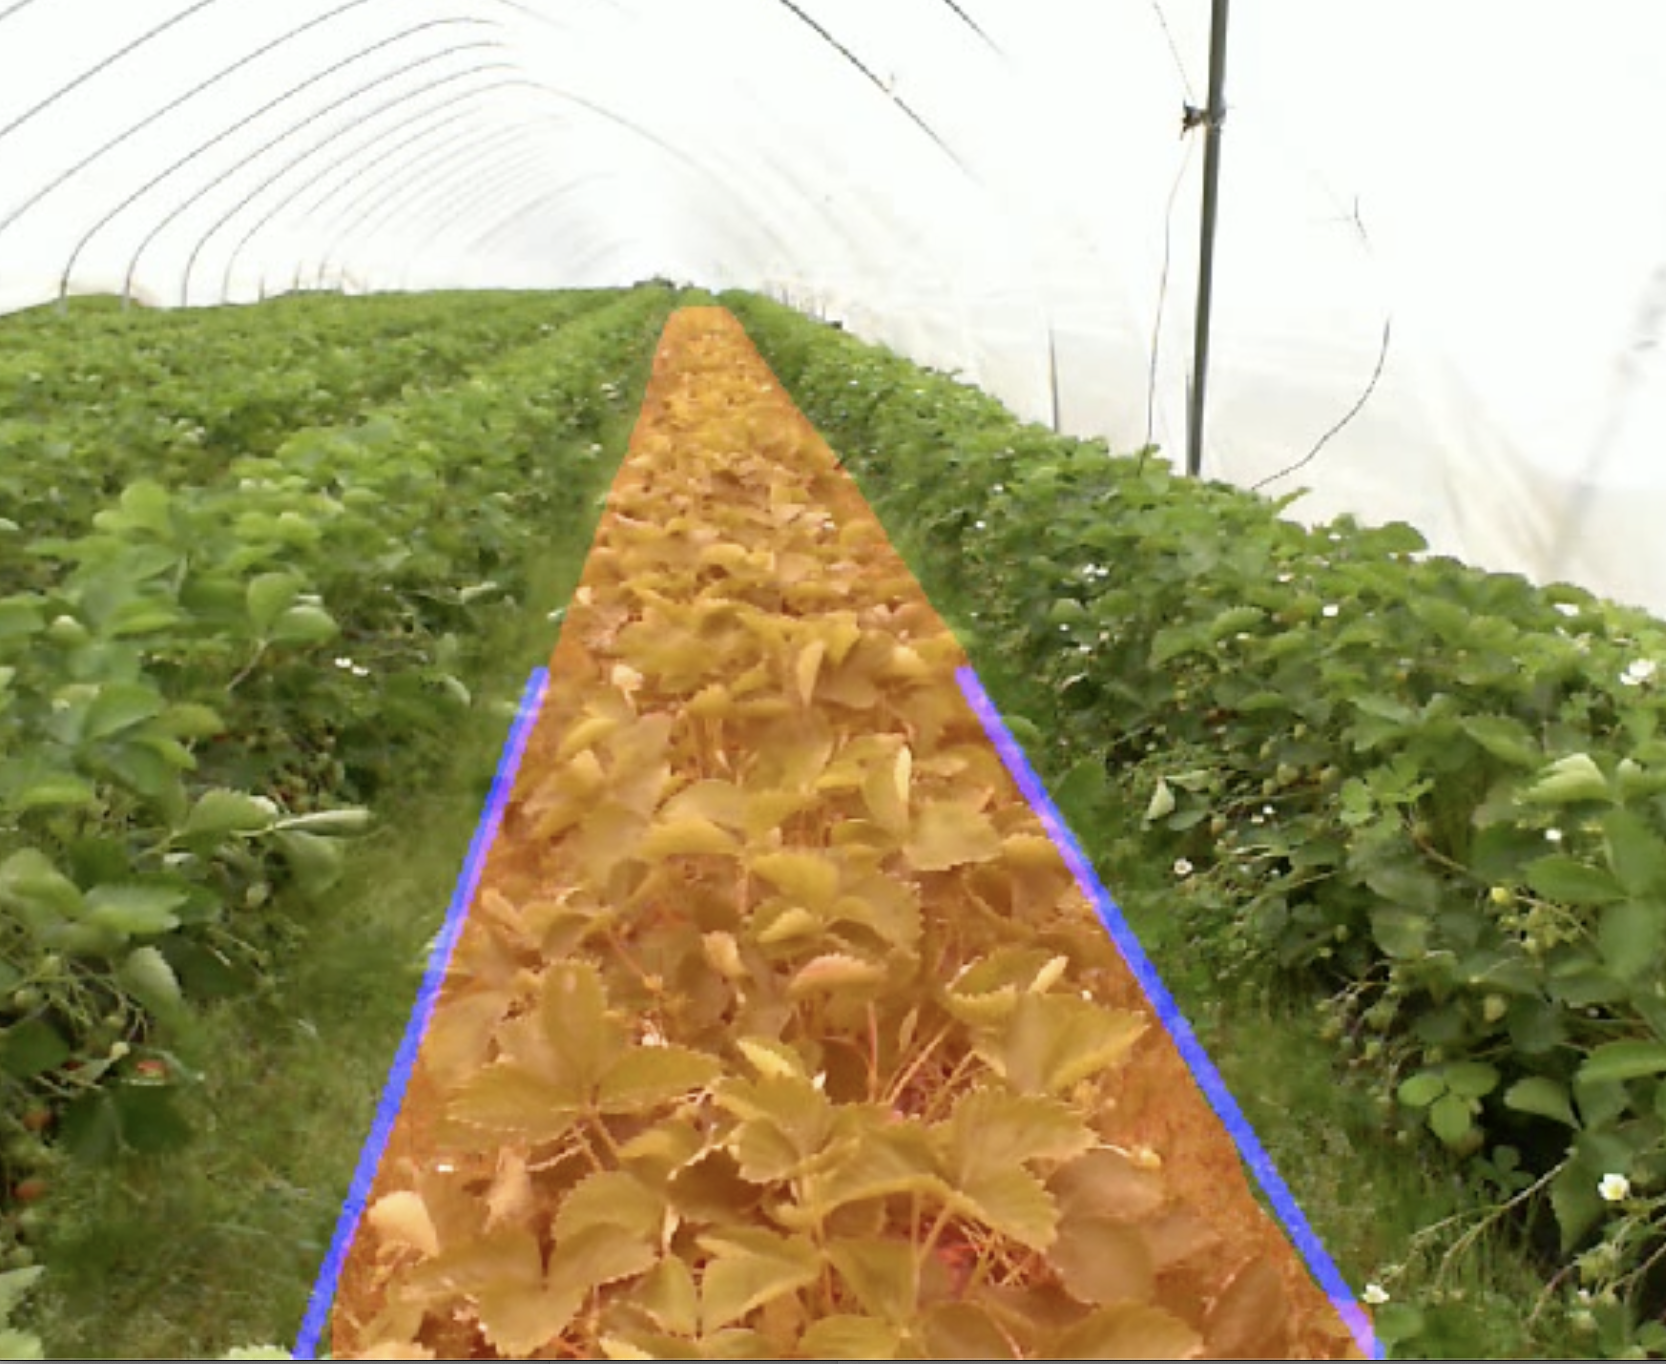
\includegraphics[width=0.7\textwidth]{Bilder/lane}
\end{center}
%\vspace{0.5cm}
\vspace{0.5cm}
}
\author{Joaquin Arias}


\lhead{
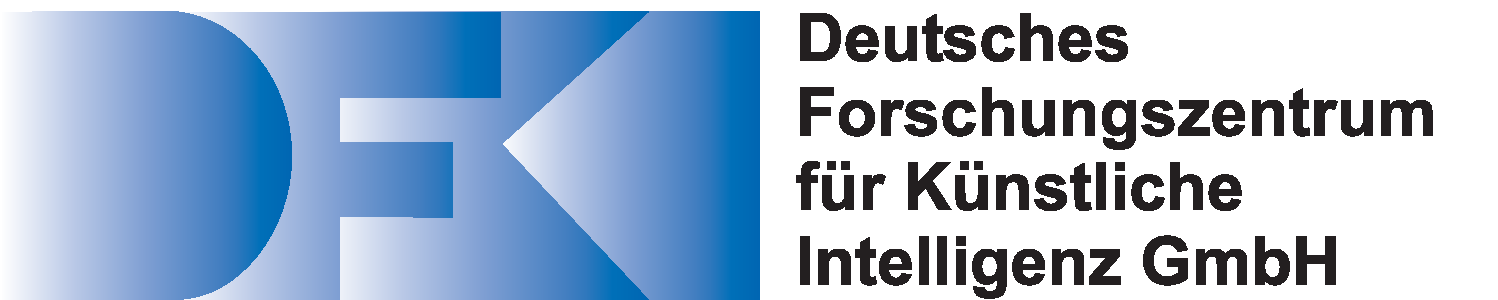
\includegraphics[width=0.7\textwidth]{DFKI_Schrift}
}


\maketitle

\vspace*{0.5cm}
\hrule
\vspace{0.5cm}

\mbox{
\parbox{.64\textwidth}{\vspace{0.5cm}
DFKI Labor Bremen\\
Robert-Hooke-Str. 5\\
28359 Bremen\\}}

\thispagestyle{fancy}

%%%%%%%%%%%%%%%%%%%%%%%%%%%%%%%%%%%%%%%%%%%%
% Index of contents, tables and images
%%%%%%%%%%%%%%%%%%%%%%%%%%%%%%%%%%%%%%%%%%%%
\newpage
\headheight0pt
\headsep20pt
\footskip36pt
%\texorpdfstring{}{\pdfoutline goto name {Table of contents} {Table of contents} \pdfdest
%name {Table of contents} xyz}
\newpage
\renewcommand*\contentsname{Table of Contents}
\tableofcontents

\clearpage

%%%%%%%%%%%%%%%%%%%%%%%%%%%%%%%%%%%%%%%%%%%%
% Text
%%%%%%%%%%%%%%%%%%%%%%%%%%%%%%%%%%%%%%%%%%%%

\newpage
%% Important: Conversion to Arabic page numbers!
\pagenumbering{arabic}

%%%%%%%%%%%%%%%%%%%%%%%%%%%%%%%%%%%%%%%%%%%%
\section{Dataset Creation}

\subsection{Rosbag to Video}
The images used for training, validating and testing were obtained from rosbag files from the robot's webcam. To convert this into a video, the file \textbf{ros2bag2video.py} was modified in the following way:

\begin{description}
\item[Line 234]: 
\begin{lstlisting}[language=Python]
elif msg_encoding.find('rgb8') != -1 or 
      msg_encoding.find('8UC3') != -1:
\end{lstlisting}

\item[Line 241]: 
\begin{lstlisting}[language=Python]
print('Unsupported encoding:', msg_encoding)
\end{lstlisting}

\item[Line 303 and 304]: Delete

\item[Line 306]:  
\begin{lstlisting}[language=Python]
img = self.bridge.imgmsg_to_cv2(msg)
img = cv2.rotate(img, cv2.ROTATE_180)
\end{lstlisting}

\end{description}

Then the following command was run and the images were extracted:

\begin{lstlisting}[language=sh]
python3 ros2bag2video.py --topic /video_frames /path/to/bag/
\end{lstlisting}
The bag files and the python script must be in the same directory.
The used videos for the datasets creation were: \textbf{rosbag2\_2022\_05\_11-15\_10\_47} and \textbf{exp5/rosbag2\_2022\_05\_11-15\_39\_43}.

In order to use only good quality images, a laplacian filter was applied to the images to determine which ones were blurry. For this, run the \textbf{detect.py} script:

\begin{lstlisting}[language=sh]
python detect.py /path/to/blurry/folder /path/to/output/folder 
--threshold 500
\end{lstlisting}

\subsection{Labeling}
There exist several software that can be used for labeling. However, in this case, the \href{https://supervisely.com/}{Supervisely Platform} was used. 
\subsubsection*{Procedure:}
First, create an account in Supervisely. Then, to upload the images, click on the cloud icon.
\begin{center}
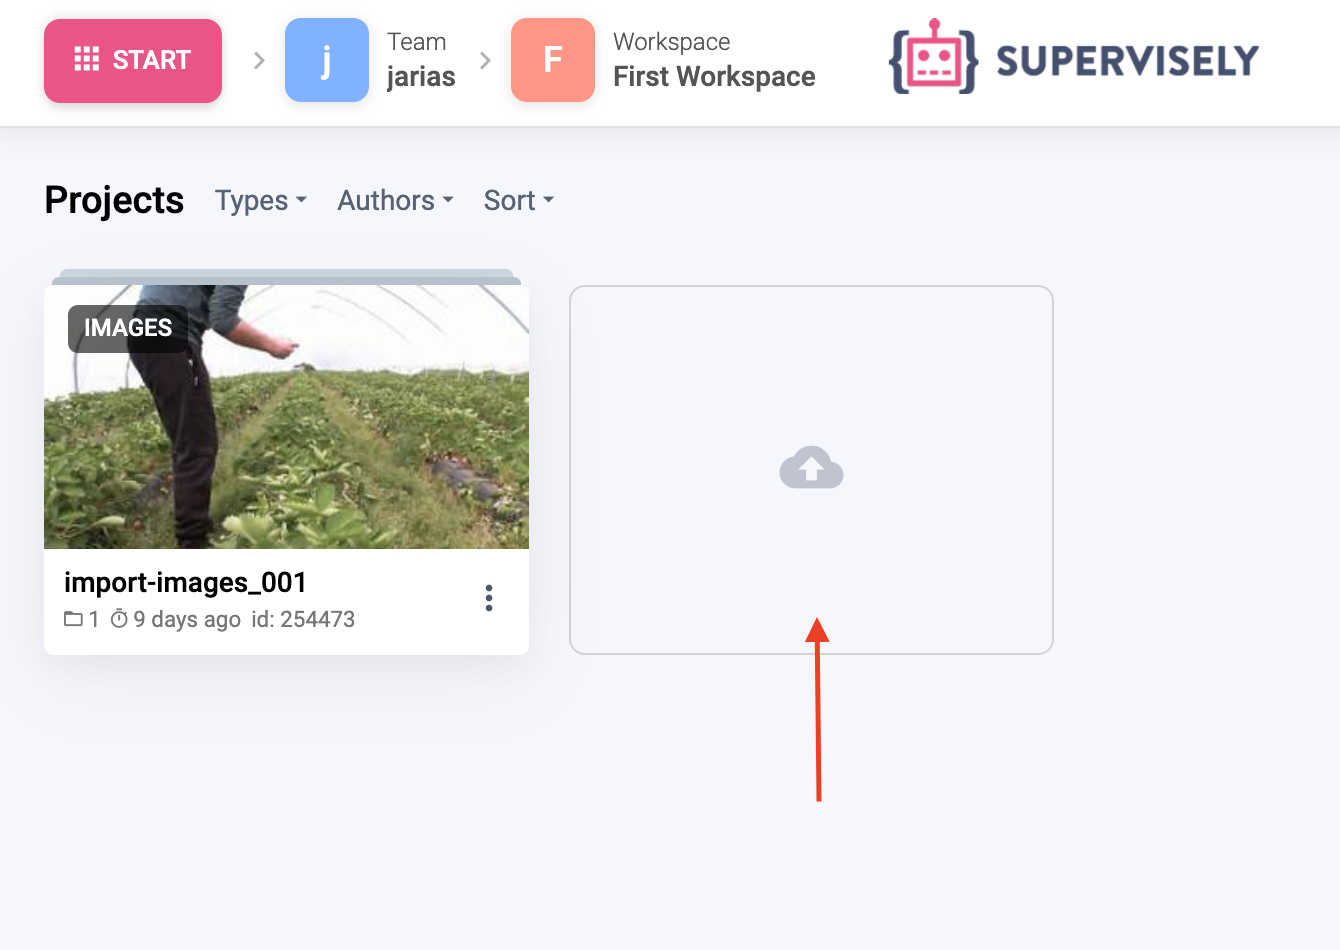
\includegraphics[width=1.0\textwidth]{Bilder/upload_1}
\end{center}

Choose \textbf{Import Images}
\begin{center}
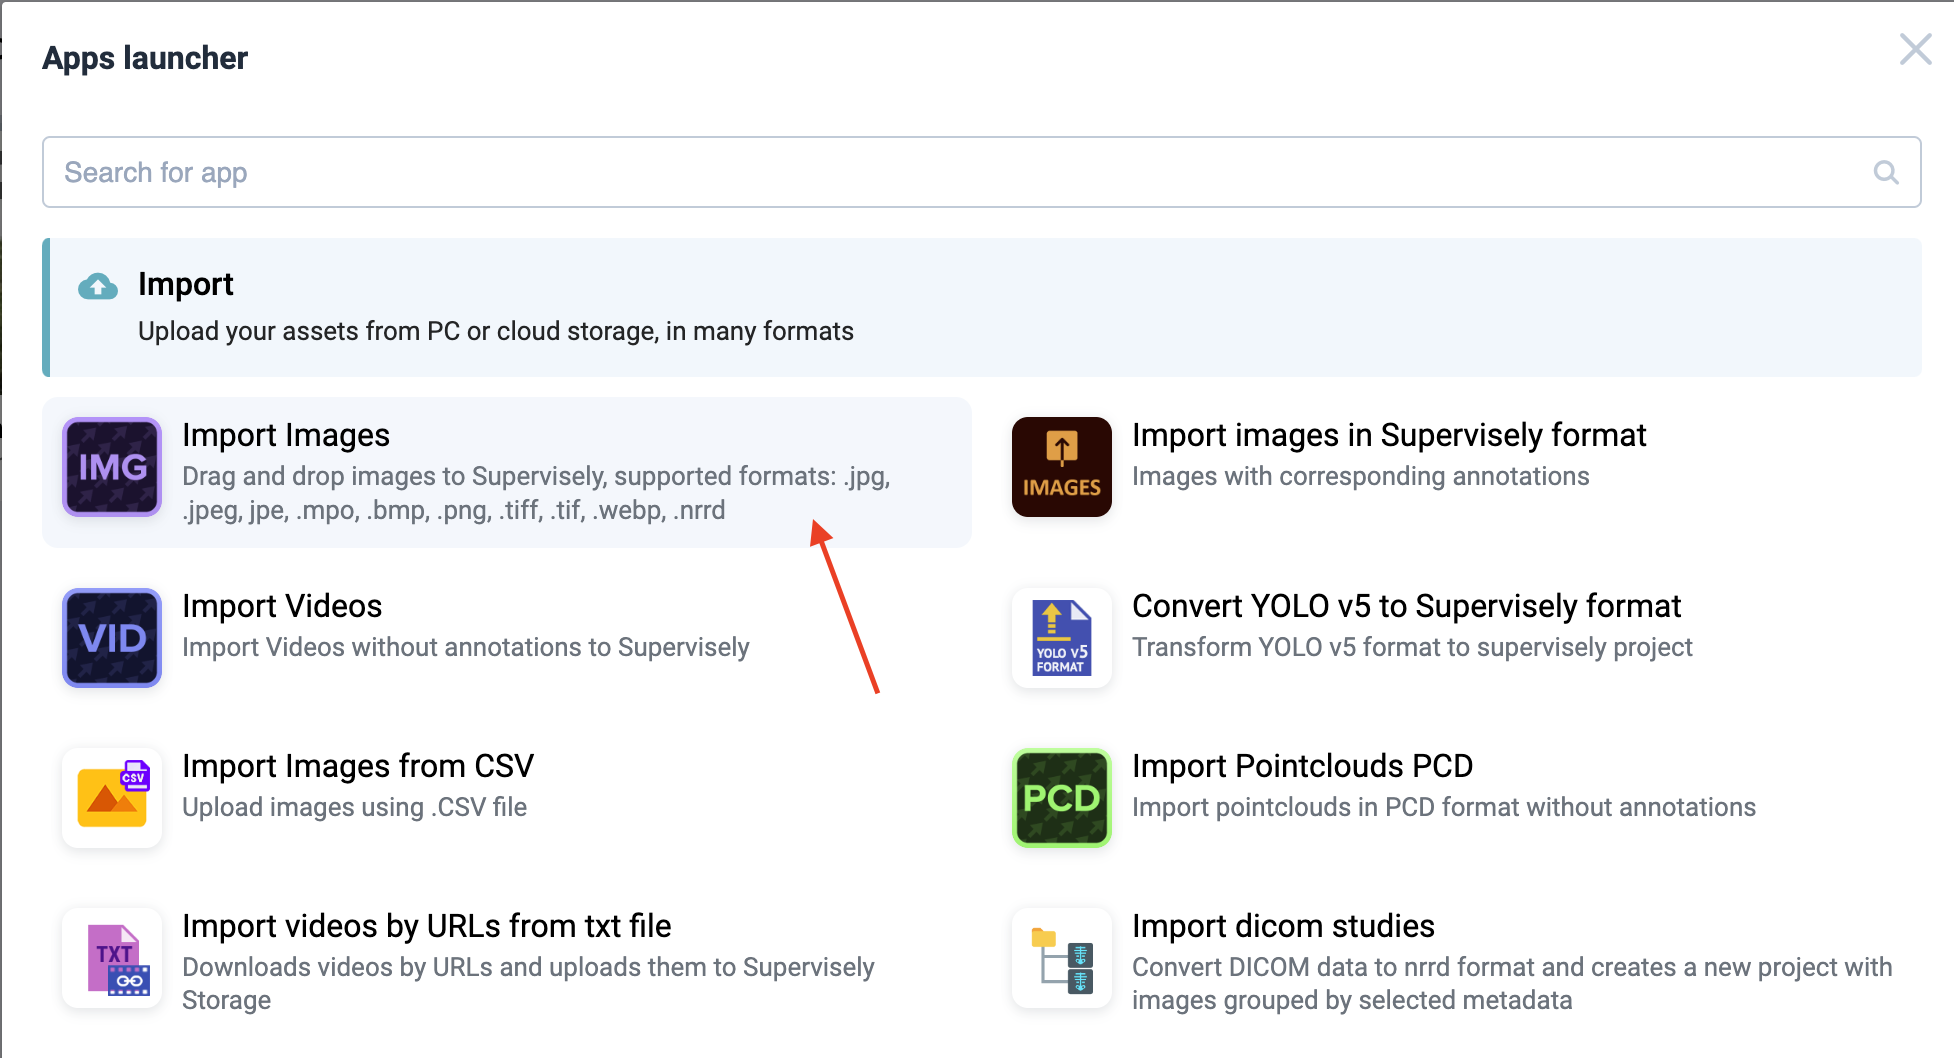
\includegraphics[width=1.0\textwidth]{Bilder/upload_2}
\end{center}

Add all the non-blurry images previously filtered and click \textbf{RUN}.

\begin{center}
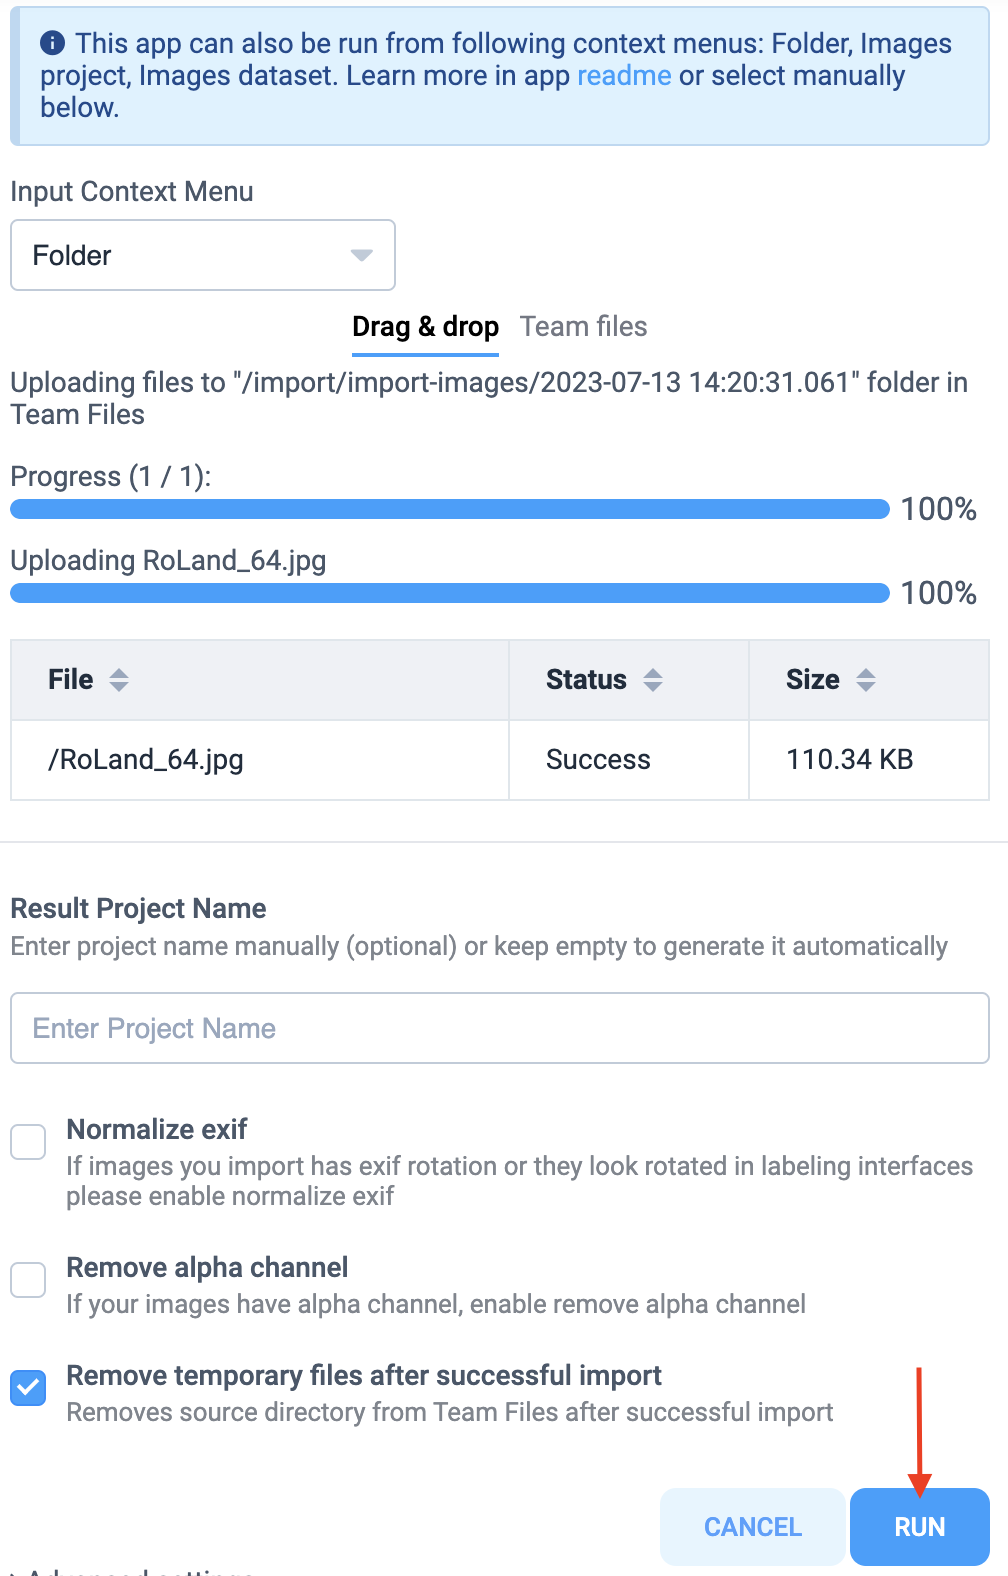
\includegraphics[width=0.6\textwidth]{Bilder/upload_3}
\end{center}
\newpage

Once it finished uploading, click on the project and choose \textbf{Advanced image labeling toolbox}.
\begin{center}
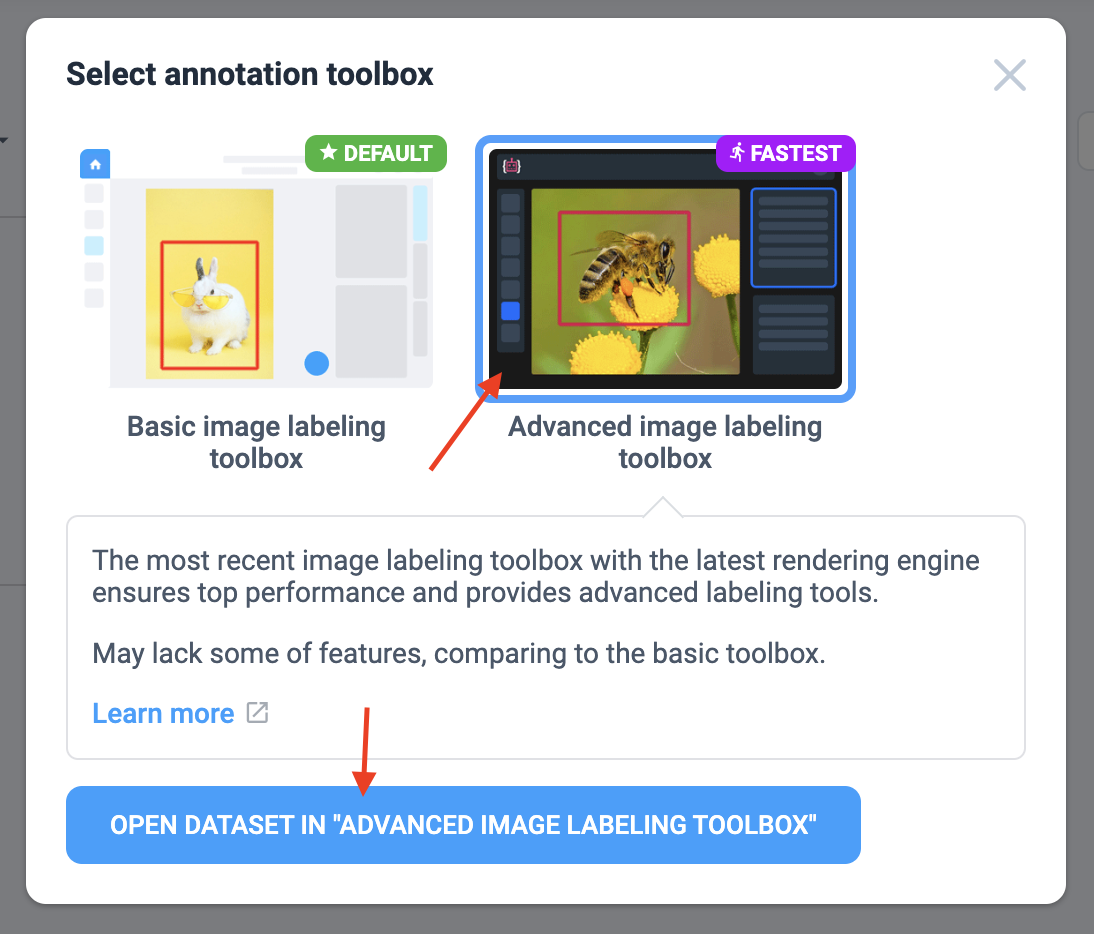
\includegraphics[width=1.0\textwidth]{Bilder/upload_4}
\end{center}
\newpage

Click on the polygon option and create a class.

\begin{center}
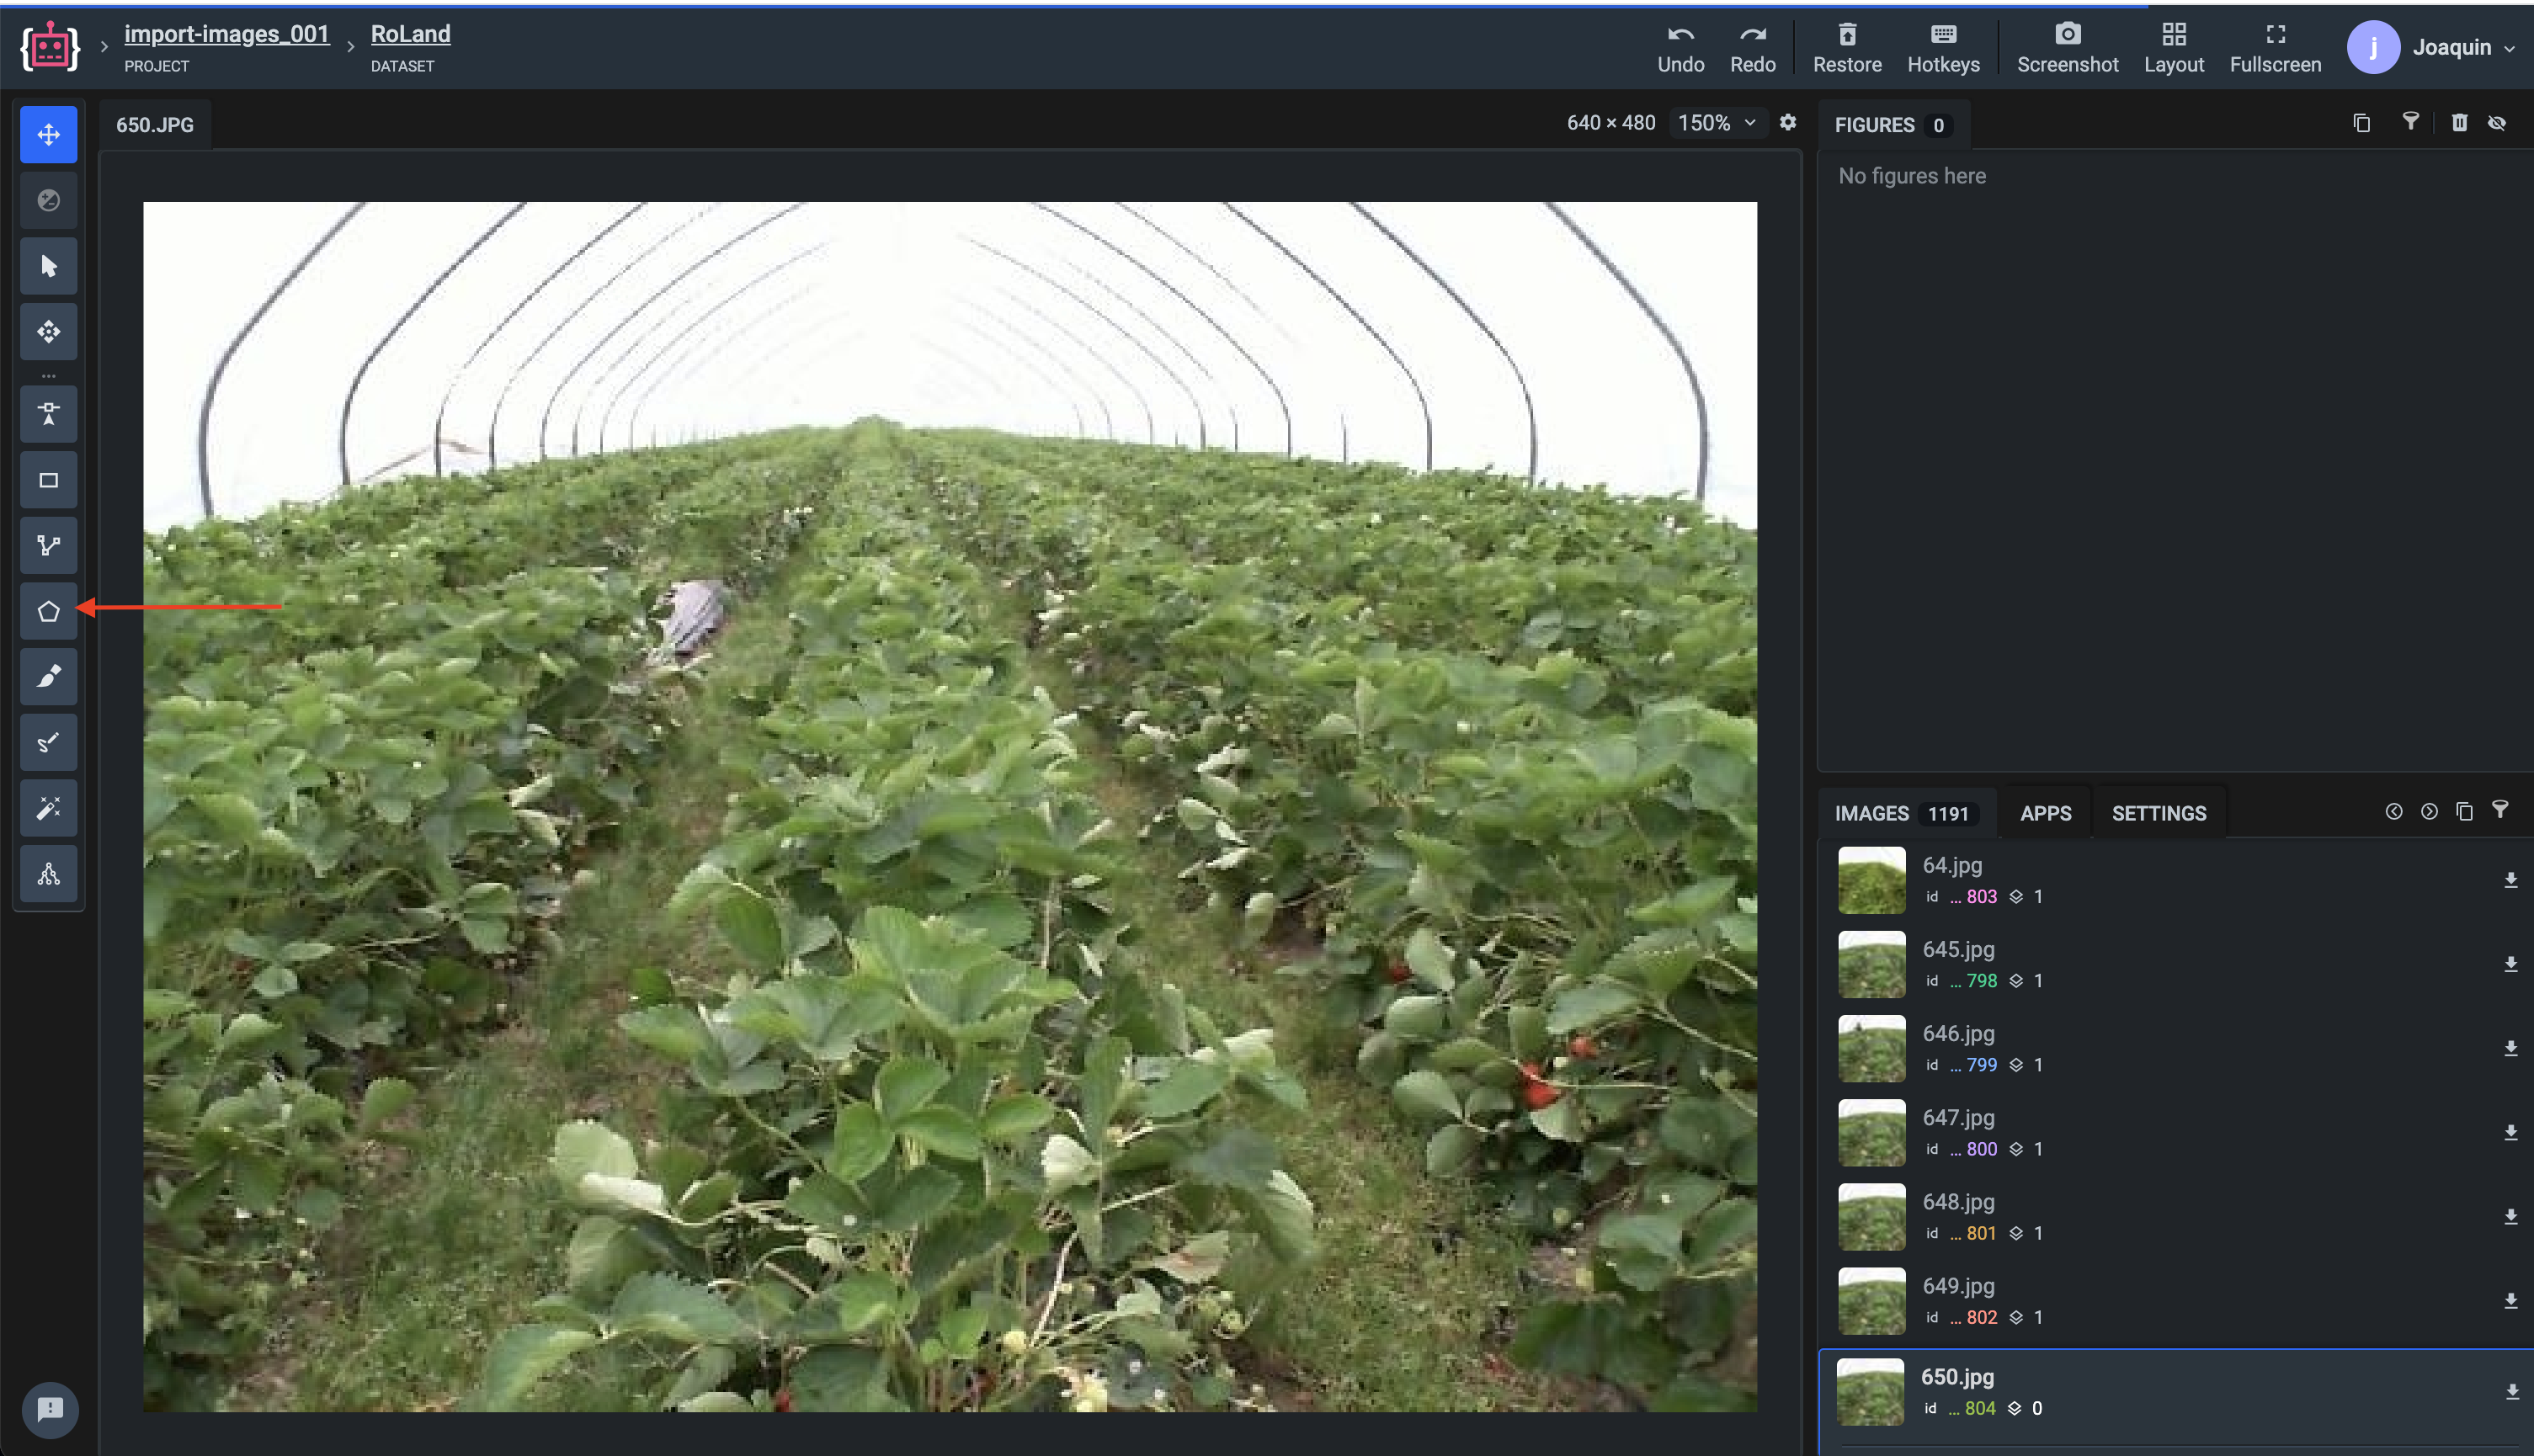
\includegraphics[width=1.0\textwidth]{Bilder/upload_5}
\end{center}

\begin{center}
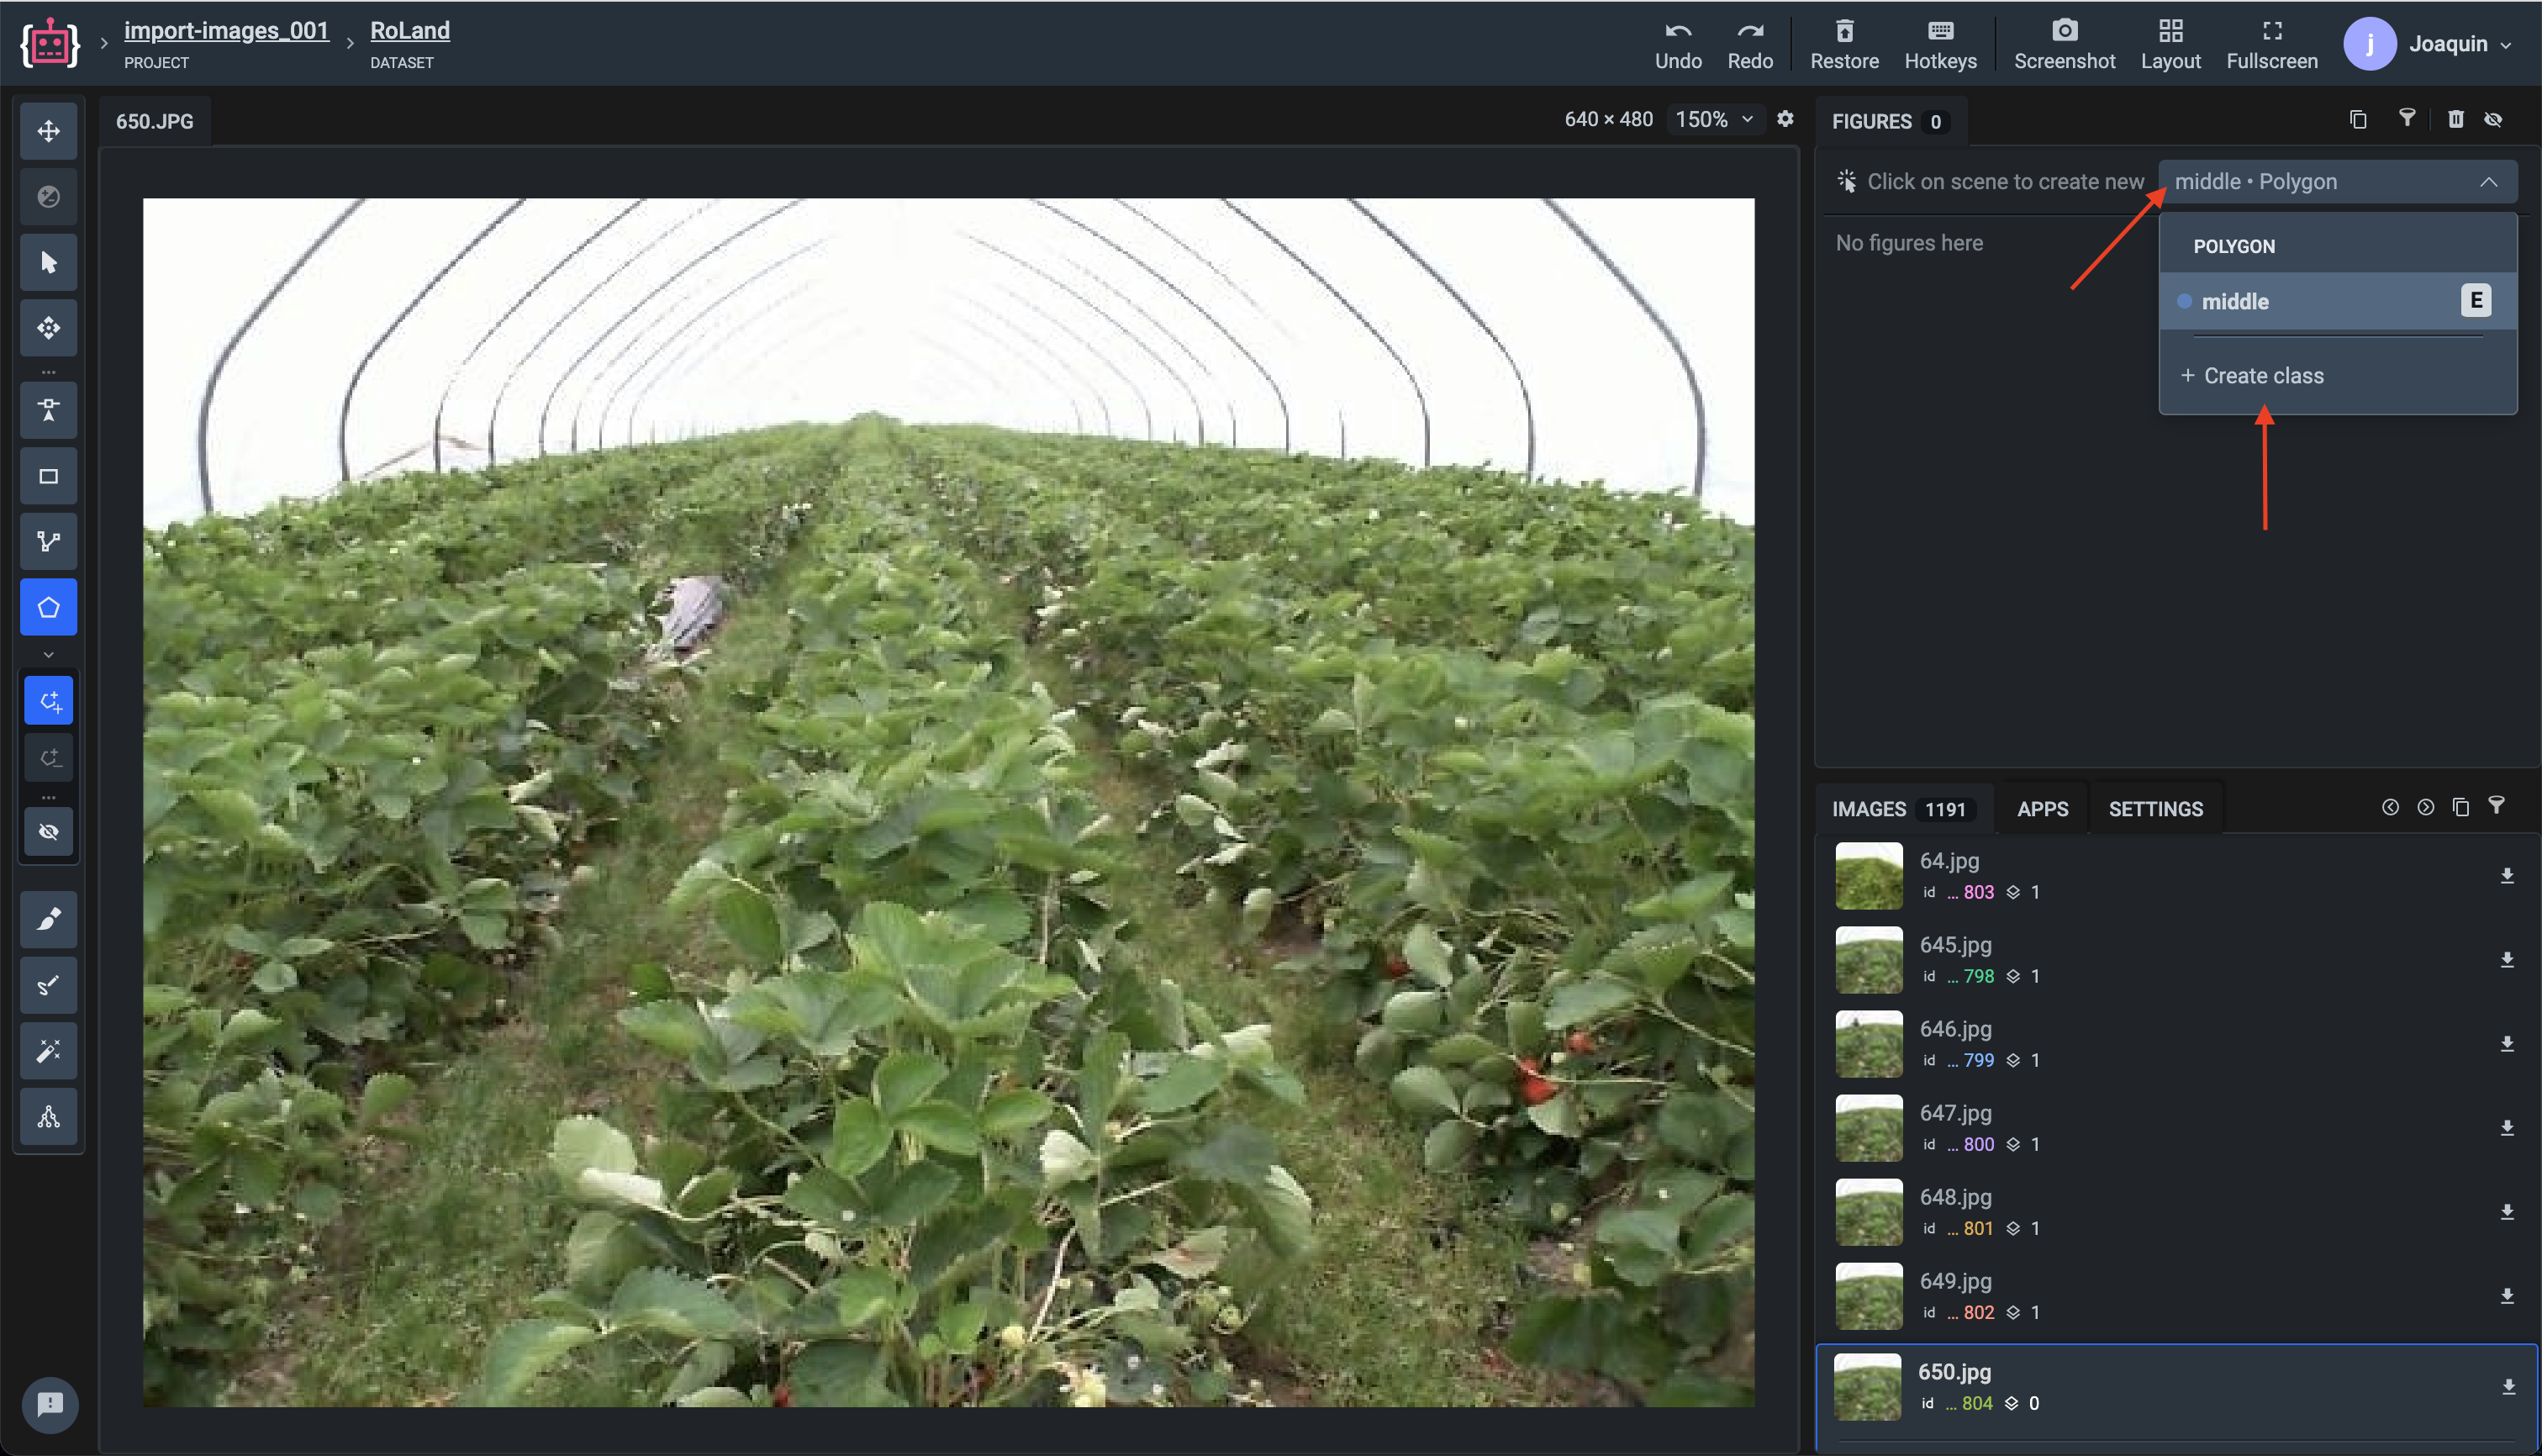
\includegraphics[width=1.0\textwidth]{Bilder/upload_6}
\end{center}

\begin{center}
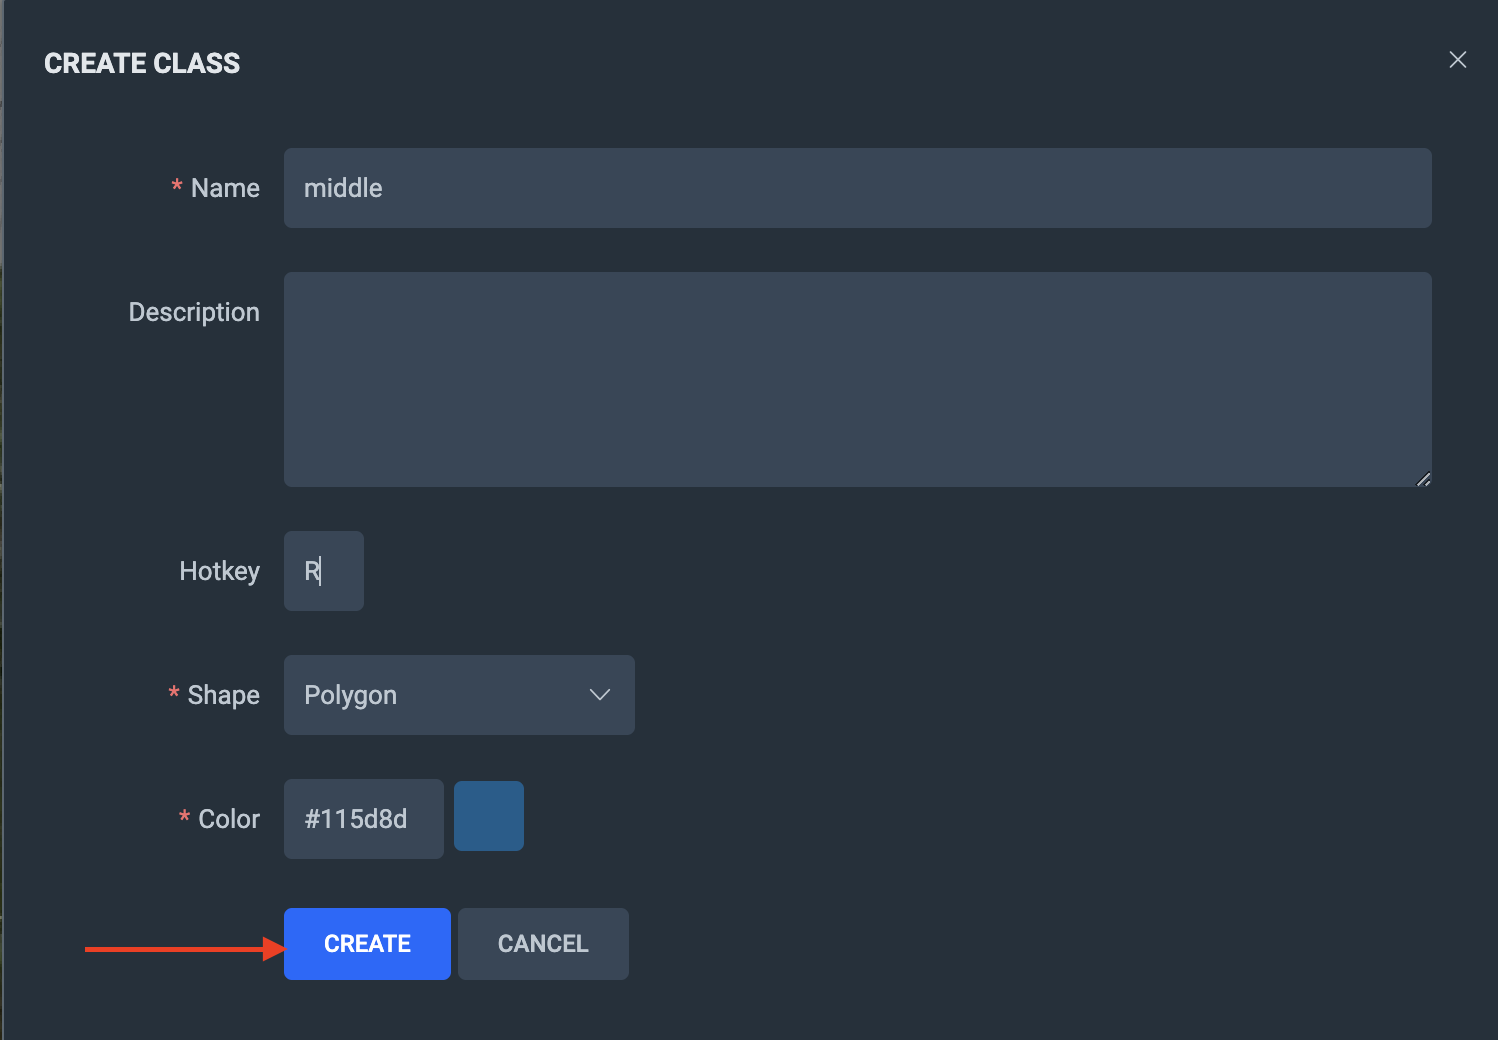
\includegraphics[width=1.0\textwidth]{Bilder/upload_7}
\end{center}

Use the mouse to create the labels around the object to label (in this case, middle lane). Press SPACE to finish the label.
\begin{center}
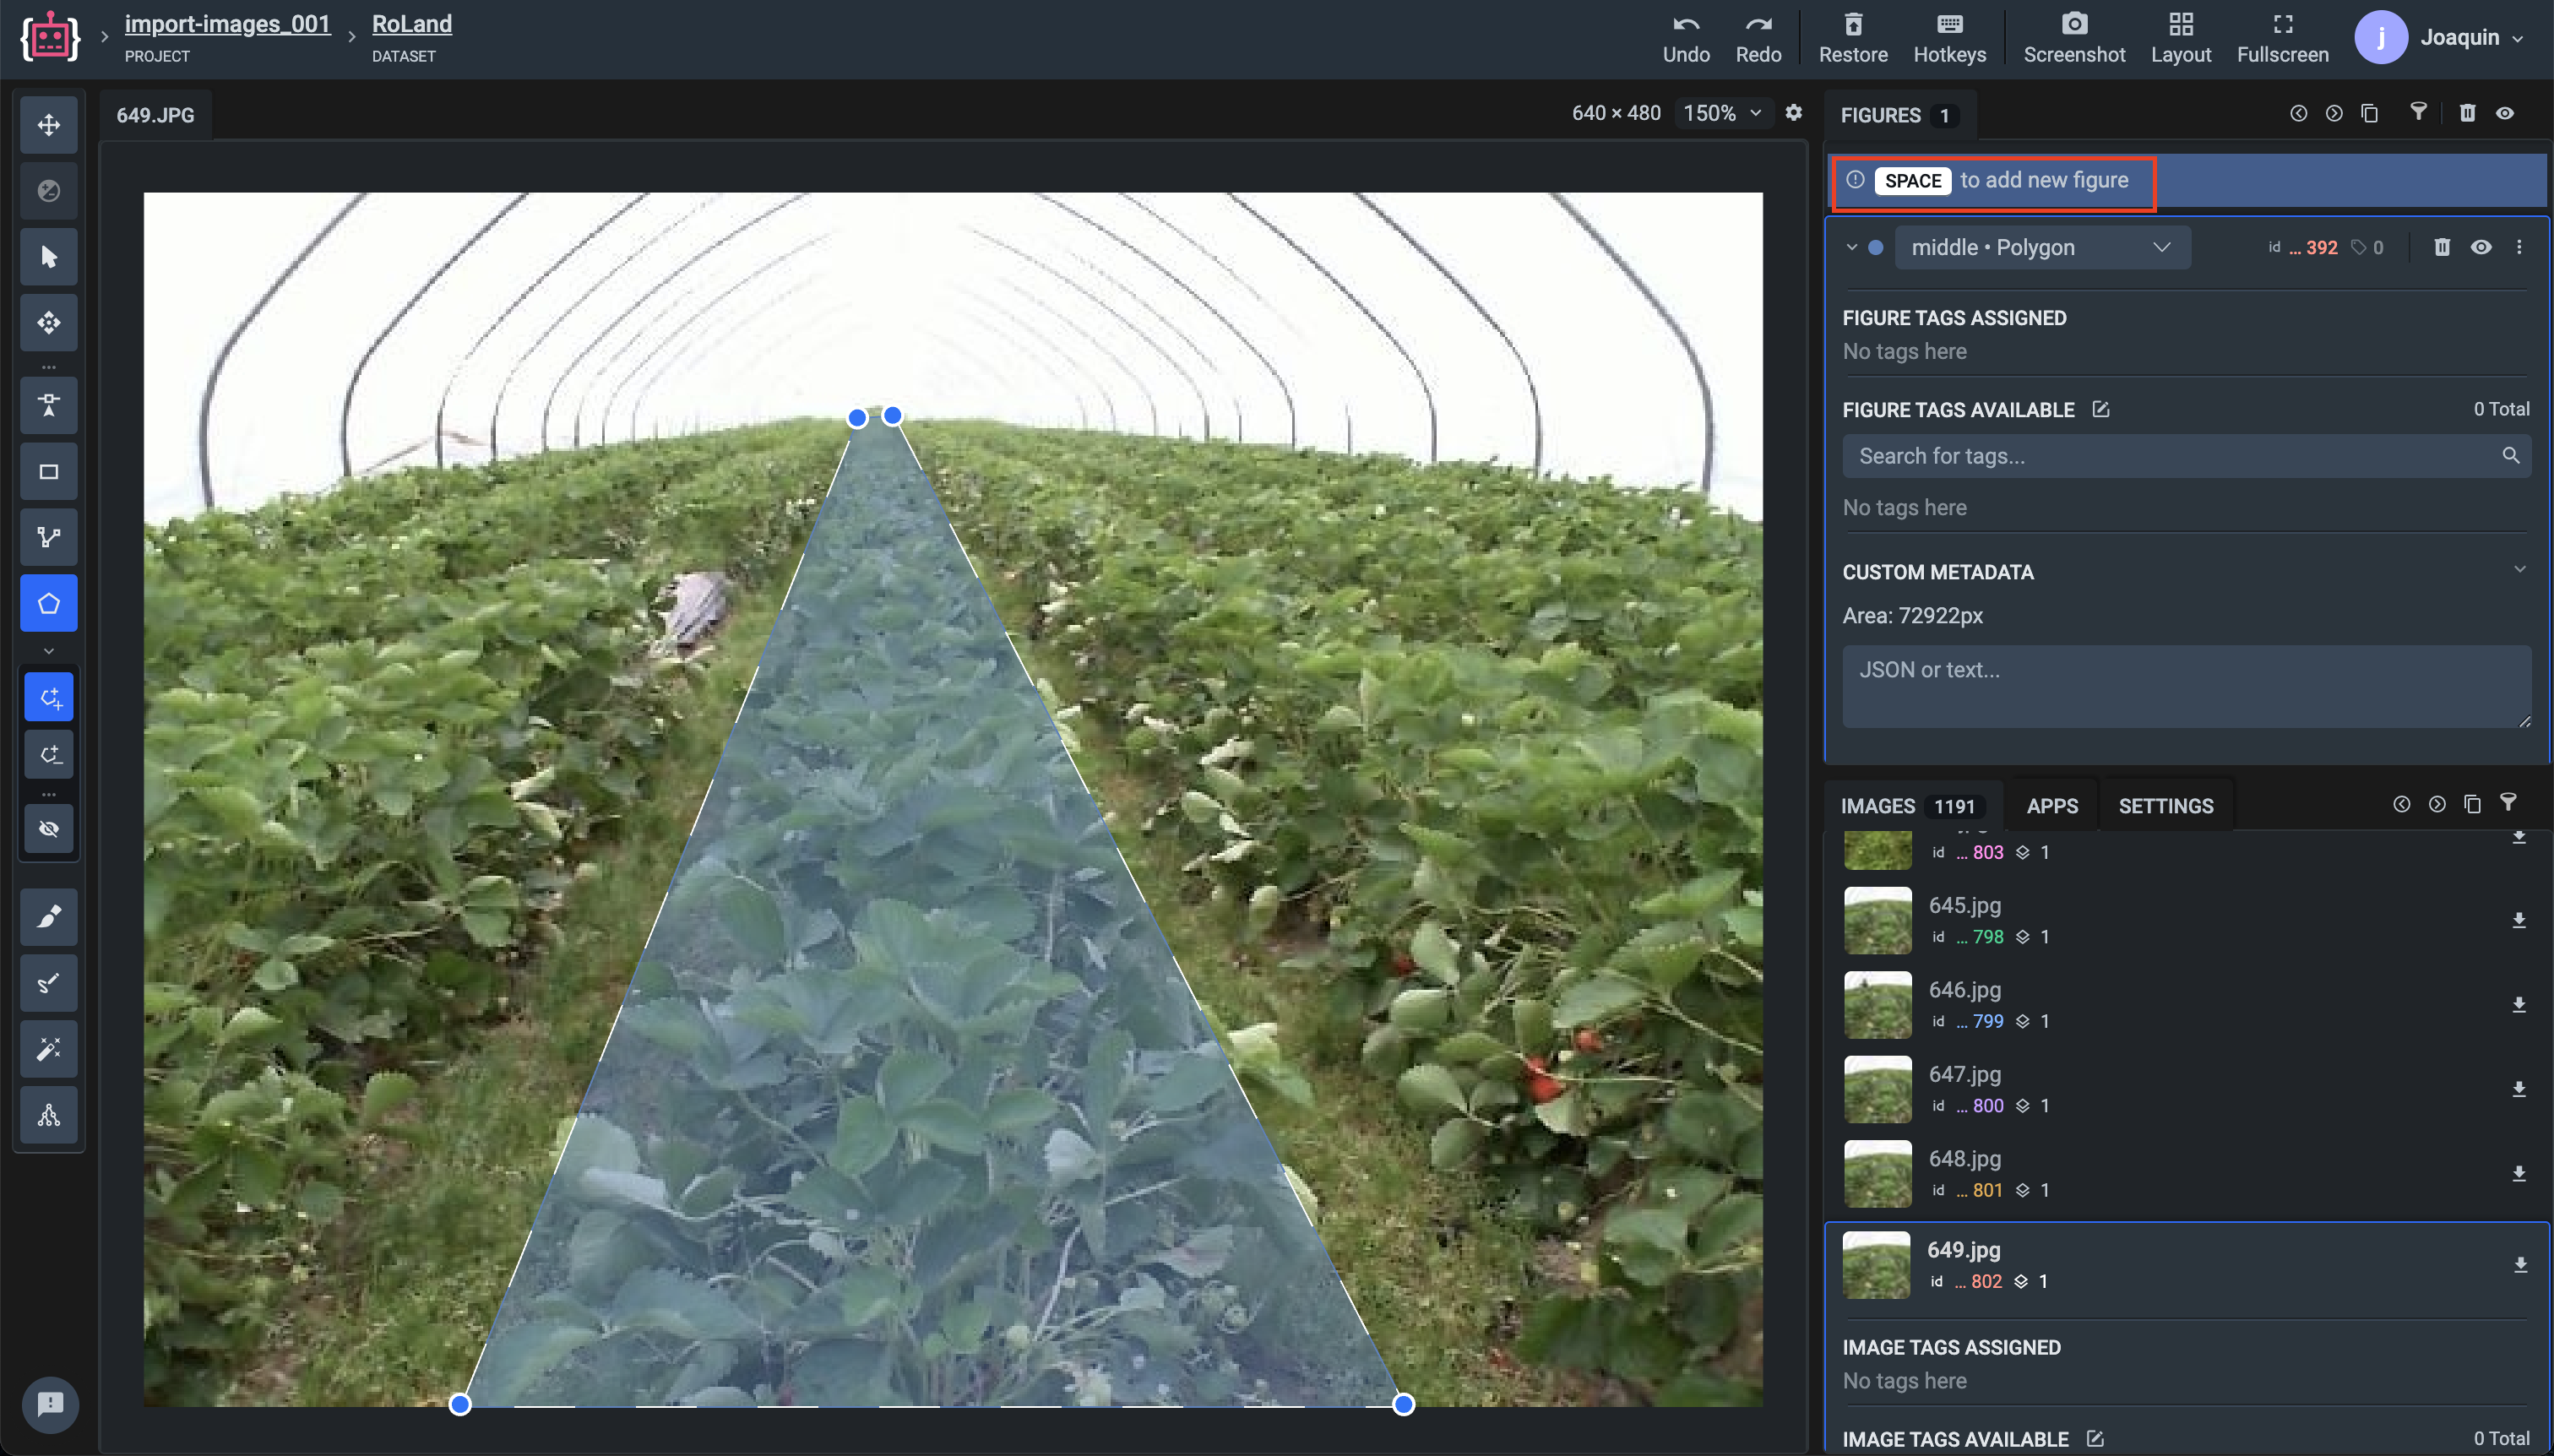
\includegraphics[width=1.0\textwidth]{Bilder/upload_8}
\end{center}
\newpage

Once all the images have been labeled, go back to the project page and click on \textbf{Export to YOLOv8 format}:
\begin{center}
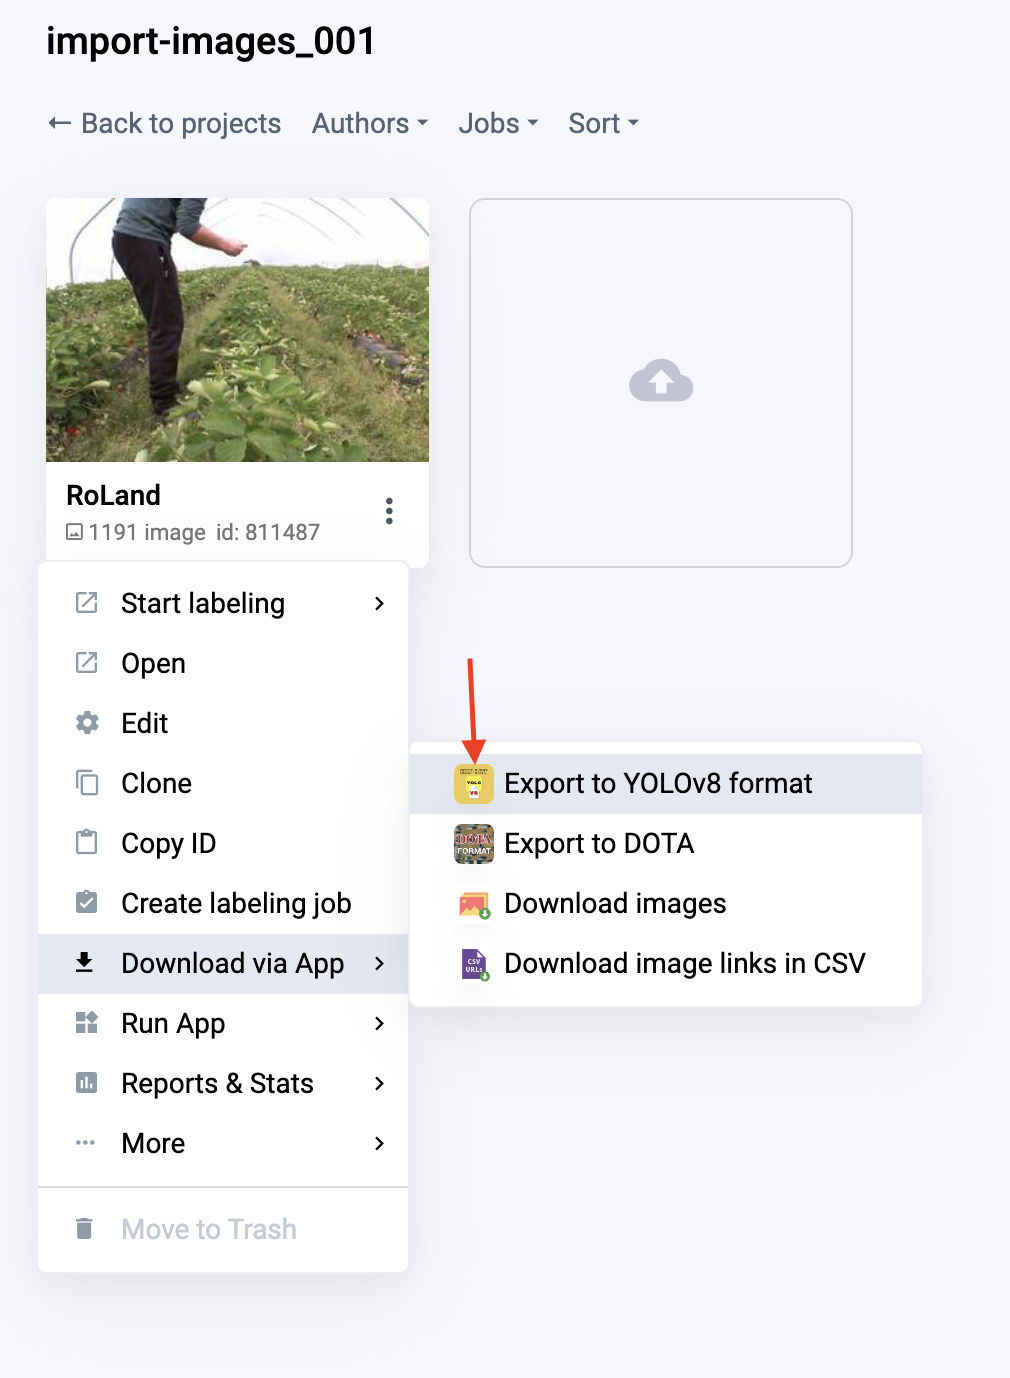
\includegraphics[width=0.6\textwidth]{Bilder/upload_10}
\end{center}
Download the generated file and it should contain the images, labels, and the \textbf{data\_config.yaml} file.


\subsection{Dataset Processing}
\subsubsection*{Removing non-labeled images:}
If not all the images were labeled, run the script \textbf{delete\_non\_labeled\_imgs.py} replacing \textbf{path/to/folder} with the path to the exported folder.

\subsubsection*{Creating Datasets:}
To create the training, validation and testing datasets, run the \textbf{create\_datasets.py} script:
\begin{lstlisting}[language=sh]
python create_datasets.py /path/to/exported/folder 
/path/to/output/dataset/folder 90
\end{lstlisting}
With this command, 90\% of the data is going to be for training, 5\% for validating, and 5\% for testing.
\newpage
\section{YOLO}
YOLO (You Only Look Once) is a real-time object detection algorithm that predicts bounding boxes and class probabilities directly from images or videos. In this case, YOLOv8 was used. This is the latest version of the model for real-time object detection and image segmentation. Built upon advancements in deep learning and computer vision, YOLOv8 offers unparalleled speed and accuracy. YOLOv8 brings new features and improvements, enhancing its performance, flexibility, and efficiency.

\subsection{Training}
\subsubsection*{Configuration File}
Open the \textbf{data\_config.yaml} and change it to:
\begin{lstlisting}[language=XML]
path: ../datasets 
train: images/train  
val: images/val  
test: images/test

names:
  0: middle
\end{lstlisting}


The pre-trained model \textbf{yolov8n-seg.pt} was used for training. Just replace the data path to the path of the config file. There were several training tests with different amounts of data and they can be found under training versions in GitHub. However, the best performance was the model trained with 716 images and the following hyperparameters:
\begin{lstlisting}[language=XML]
epochs: 20
patience: 30
batch: 16
imgsz: 640
pretrained: true
lr0: 0.001
lrf: 0.001
weight_decay: 0.0005
\end{lstlisting}

\subsubsection*{Training Results}


\begin{center}
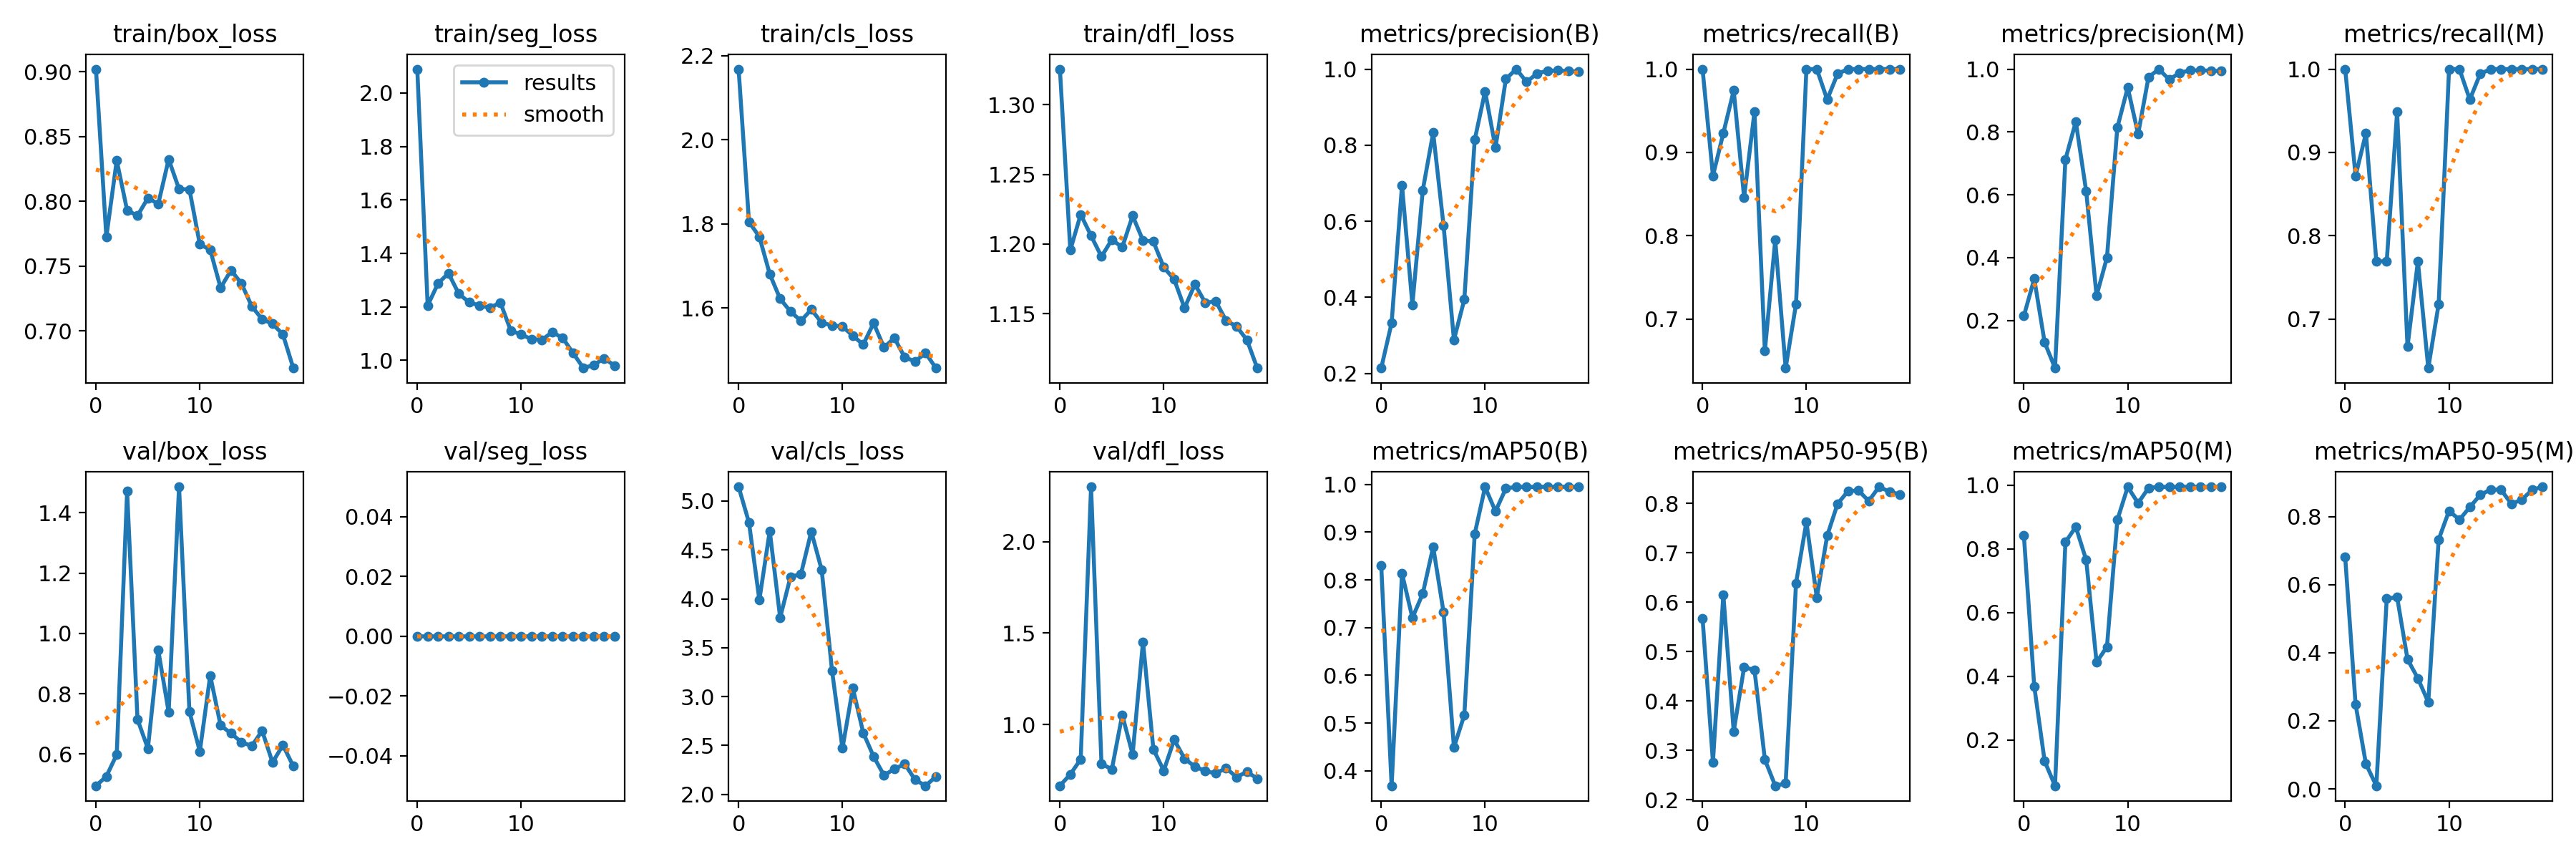
\includegraphics[width=1.0\textwidth]{Bilder/results}
\end{center}


Batch 0 labels:
\begin{center}
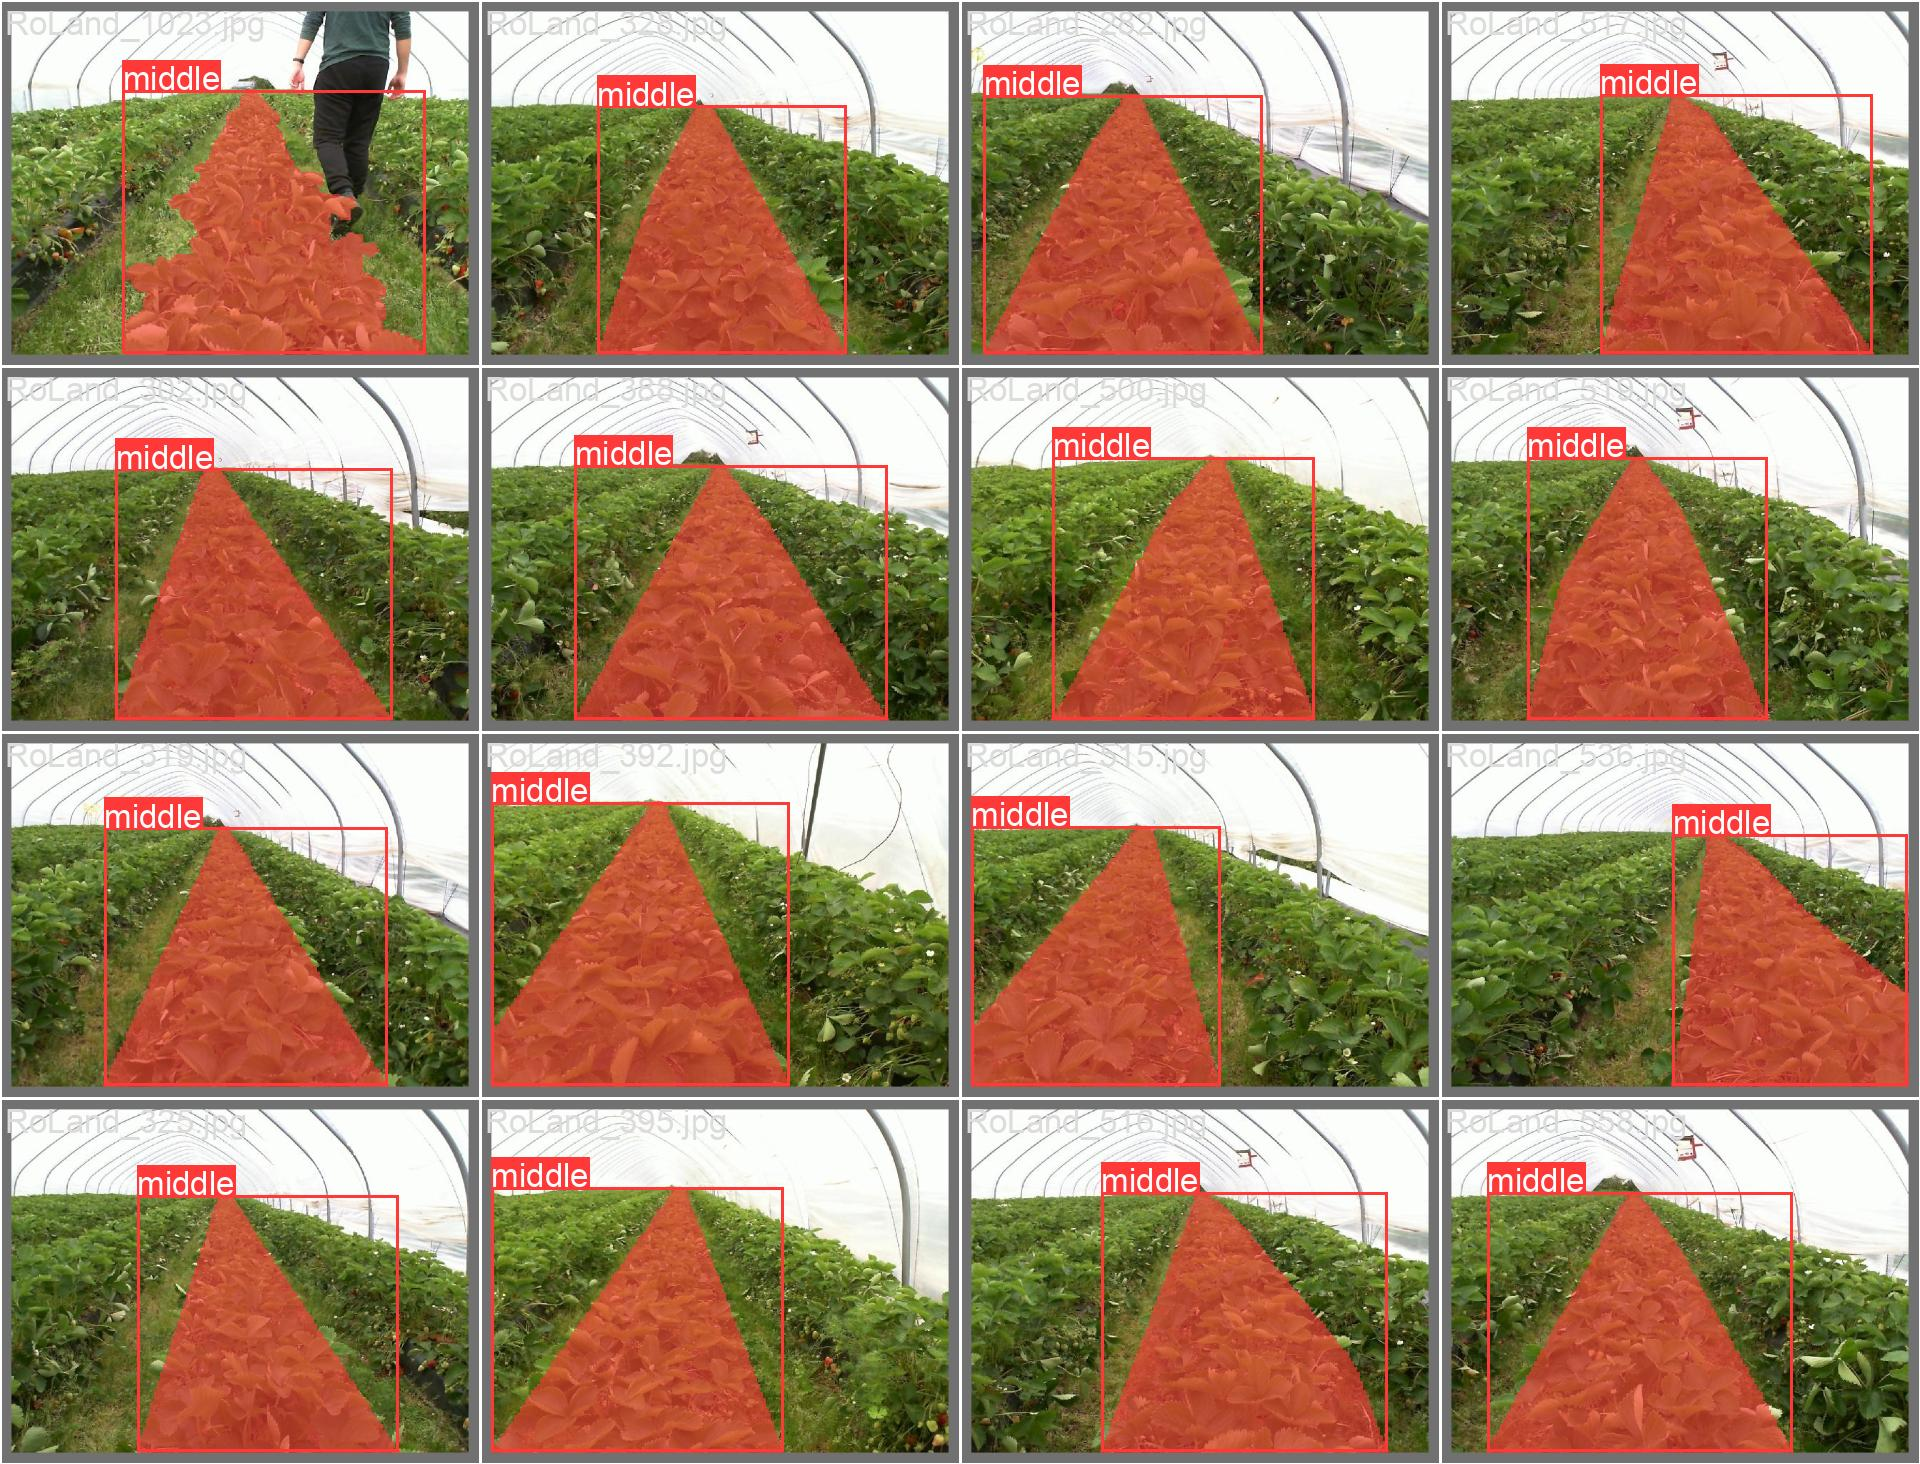
\includegraphics[width=1.0\textwidth]{Bilder/val_batch0_labels}
\end{center}
\newpage

Batch 0 predictions:
\begin{center}
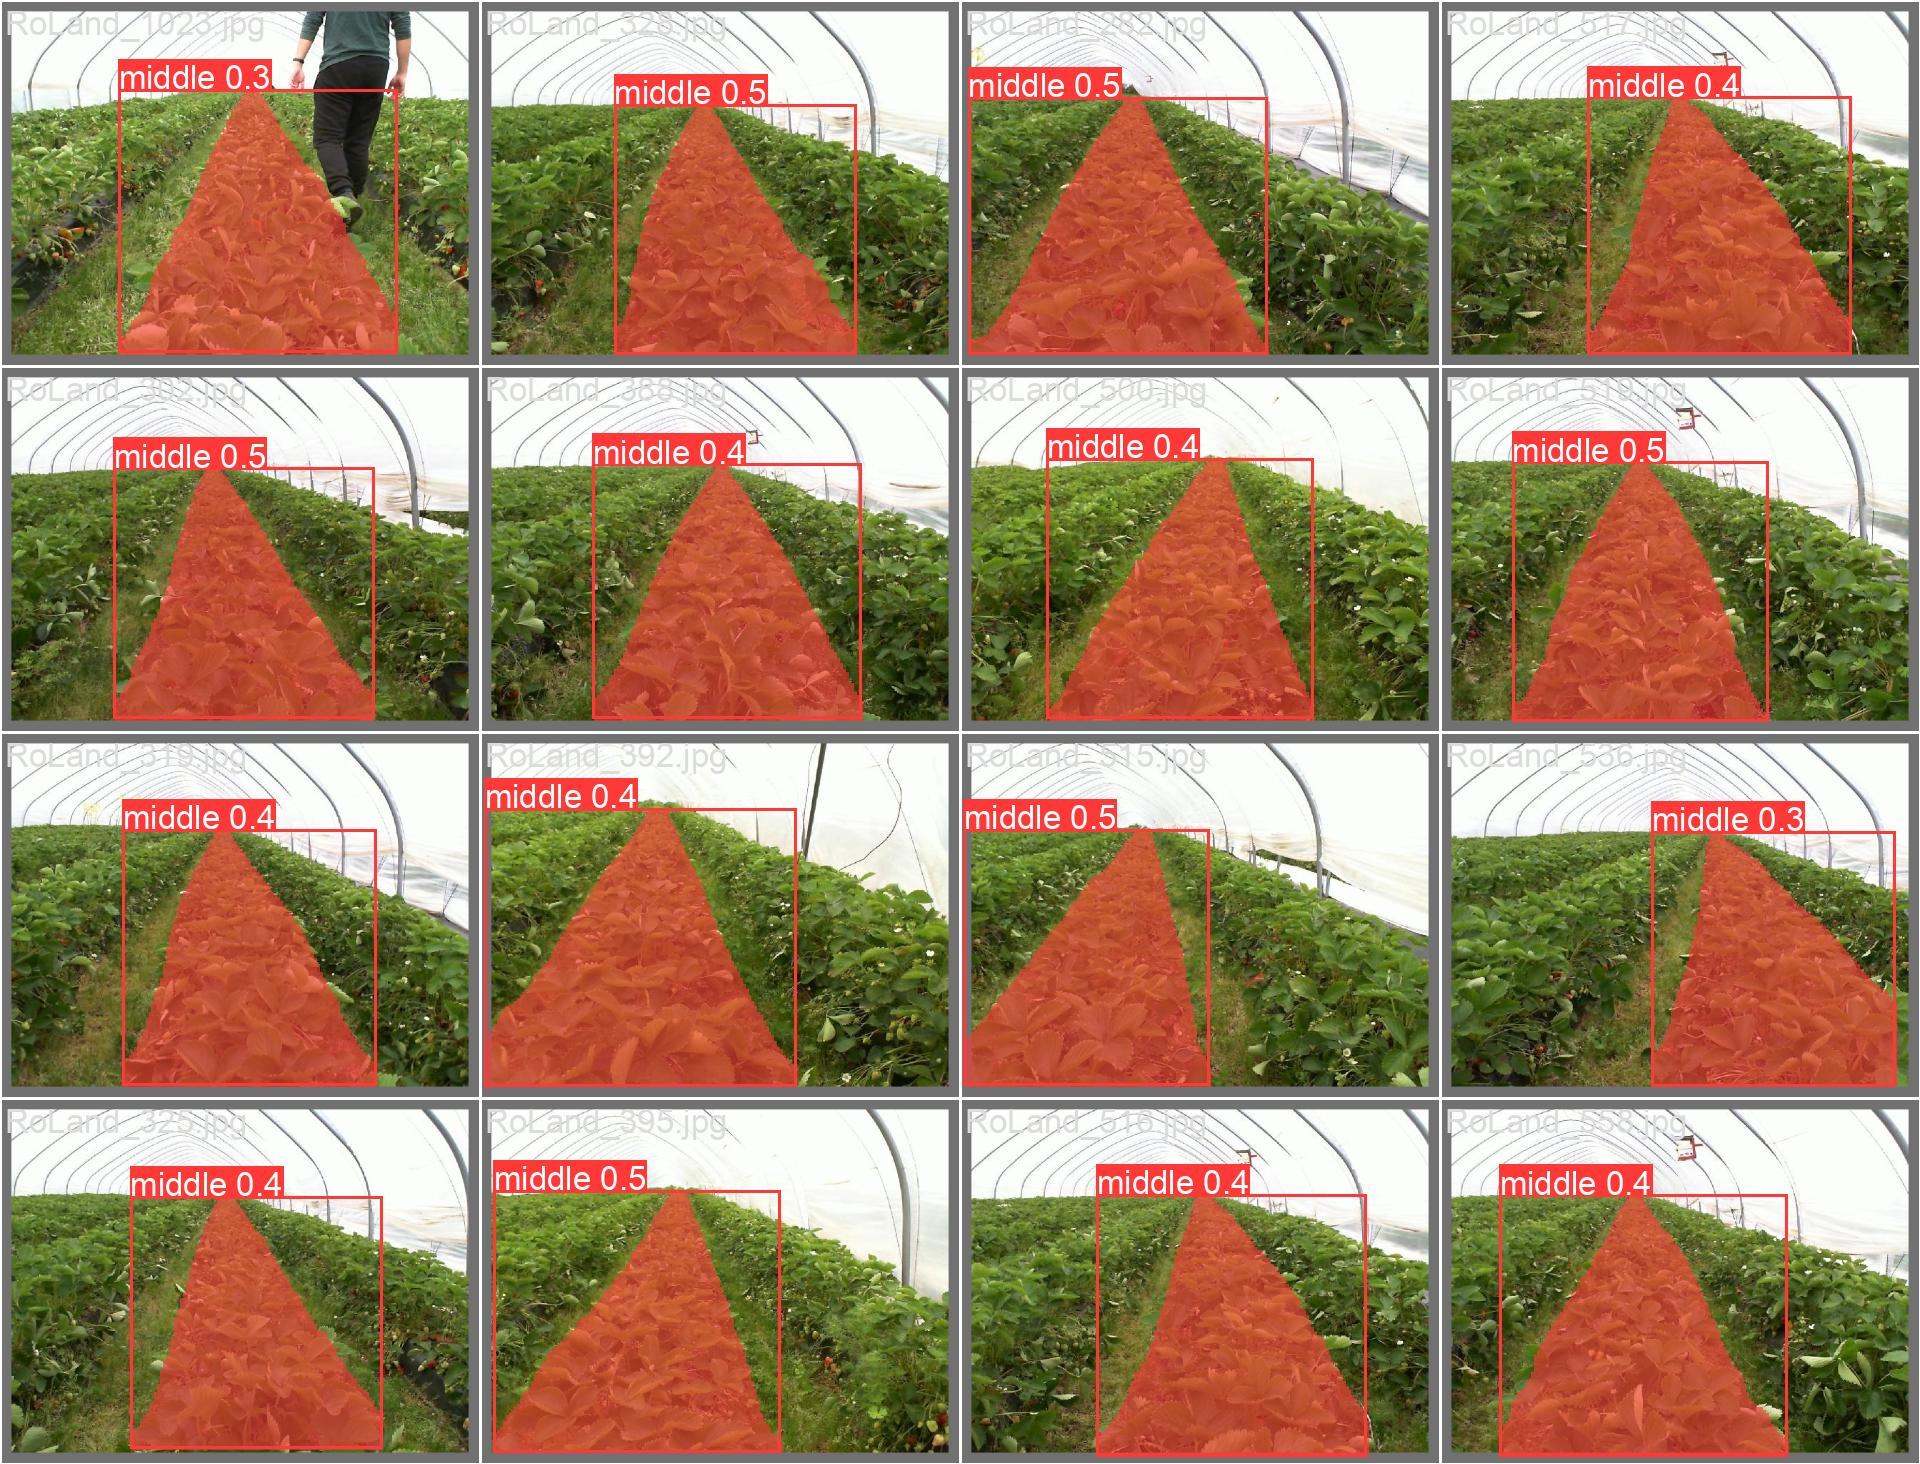
\includegraphics[width=1.0\textwidth]{Bilder/val_batch0_pred}
\end{center}

The best model is saved in \textbf{'runs/segment/train/weights/best.pt'}

\subsection{Prediction}
To predict the, use the \textbf{predict.py} file and replace the directory path with the path to the test folder from the datasets.
\subsection{Validation}
For validation, use the \textbf{val.py} script and load the trained model.
%%%%%%%%%%%%%%%%%%%%%%%%%%%%%%%%%%%%%%%%%%%%
\newpage

\section{Orientation and Position Detection}
Now that the lane is being detected, it is necessary to calculate its position and orientation with respect to the camera.

%%%%%%%%%%%
\subsection{Lane Borders Detection}
\subsubsection*{Mask}

First, the detection mask has to be extracted:
\begin{lstlisting}[language=Python]
# Predict with the model
model.predict(directory, max_det=1, boxes=False)

# Extract the lane region

# Predict on an image
results = model(directory) 
# Get the masks object from the results
masks = results[0].masks  
 # Get the mask corresponding to the first detected object (lane)
mask = masks.data[0].numpy() 

# Create a binary image from the mask
binary_mask = (mask > 0).astype(np.uint8) * 255
\end{lstlisting}

\begin{figure}[!h]
	\centering
	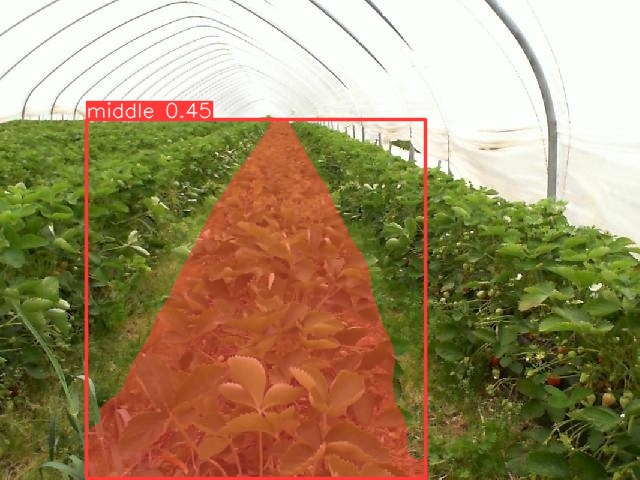
\includegraphics[width=0.5\textwidth]{Bilder/detection}%
	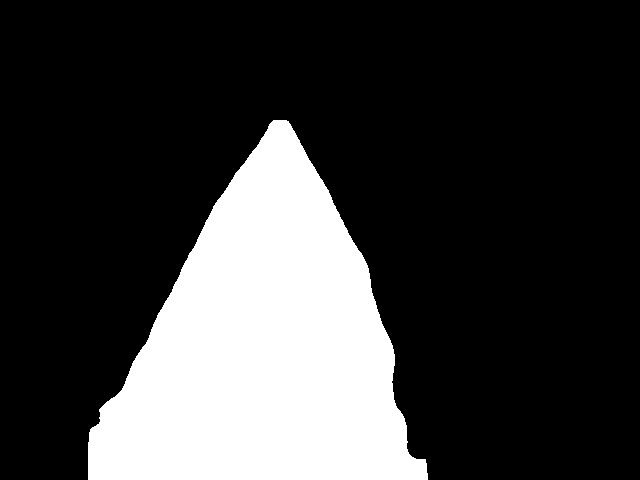
\includegraphics[width=0.5\textwidth]{Bilder/binary_mask}%
\end{figure}

\subsubsection*{Canny Edge Detection}

Now the Canny edge detector is applied to the mask:
\begin{lstlisting}[language=Python]
# Apply Canny edge detection
edges = cv2.Canny(binary_mask, 50, 150)
\end{lstlisting}

\begin{center}
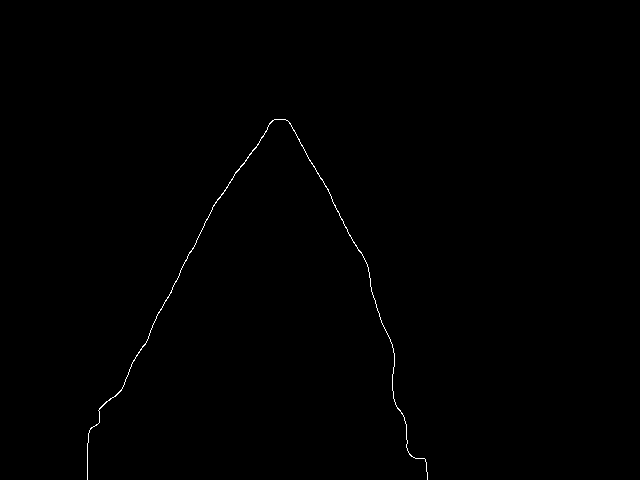
\includegraphics[width=1.0\textwidth]{Bilder/edges}
\end{center}

To detect the lines, the Hough Transform is applied:
\begin{lstlisting}[language=Python]
# Apply Hough transform to detect lines
 lines = cv2.HoughLinesP(edges, 1, np.pi / 180, 50, None, 50, 10)
\end{lstlisting}
And assign each detected line to either left or right boundaries:
\begin{lstlisting}[language=Python]
# Filter and separate lines as left and right lane boundaries
left_lines = []
right_lines = []

if lines is not None:
    for line in lines:
        x1, y1, x2, y2 = line[0]
        slope = (y2 - y1) / (x2 - x1)
        if slope < -0.5:
            left_lines.append(line[0])
        elif slope > 0.5:
            right_lines.append(line[0])

# Fit lines to left and right lane boundaries if lines 
   were detected
left_lane = np.mean(left_lines, axis=0, dtype=np.int32) 
	     if left_lines else None
right_lane = np.mean(right_lines, axis=0, dtype=np.int32) 
	     if right_lines else None
\end{lstlisting}

Then, the lines are extended and set to begin from the bottom of the image so the result looks like:
\begin{center}
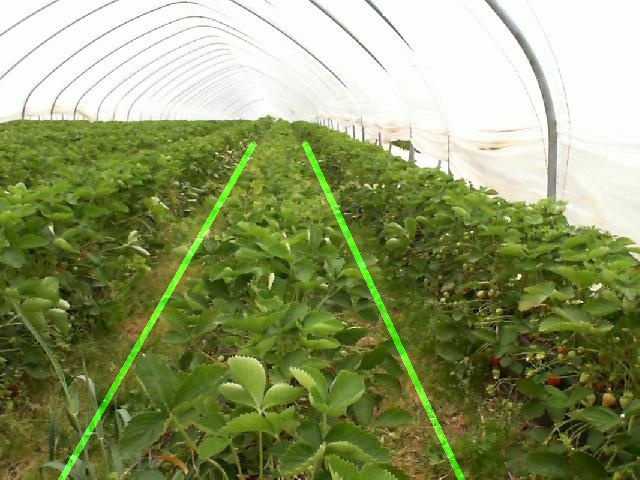
\includegraphics[width=1.0\textwidth]{Bilder/result}
\end{center}


%%%%%%%%%%%
\subsection{Middle of the Lane Determination}
After the borders have been detected, the middle of the lane is calculated:
\begin{lstlisting}[language=Python]
middle_x_bottom = int((left_lane_extended[0] + 
		right_lane_extended[0]) / 2)
middle_x_top = int((left_lane_extended[2] + 
		right_lane_extended[2]) / 2)
middle_y_bottom = y1
middle_y_top = y2
middle_slope = (middle_y_top - middle_y_bottom) / 
		(middle_x_top - middle_x_bottom)
\end{lstlisting}

%%%%%%%%%%%
\subsection{Rotation}
\subsubsection*{Description}
In order to determine the rotation of the robot with respect to the lane, the angle between the lane and the base of the image was calculated. If the angle is more than $10\degree$ off from the $y-axis$, then the text showing the angle is going to turn red. 

\begin{center}
\includegraphics[width=0.8\textwidth]{Bilder/angle}
\end{center}
\newpage

\subsubsection*{Angle Determination}
The angle is calculated using trigonometry:

\begin{center}
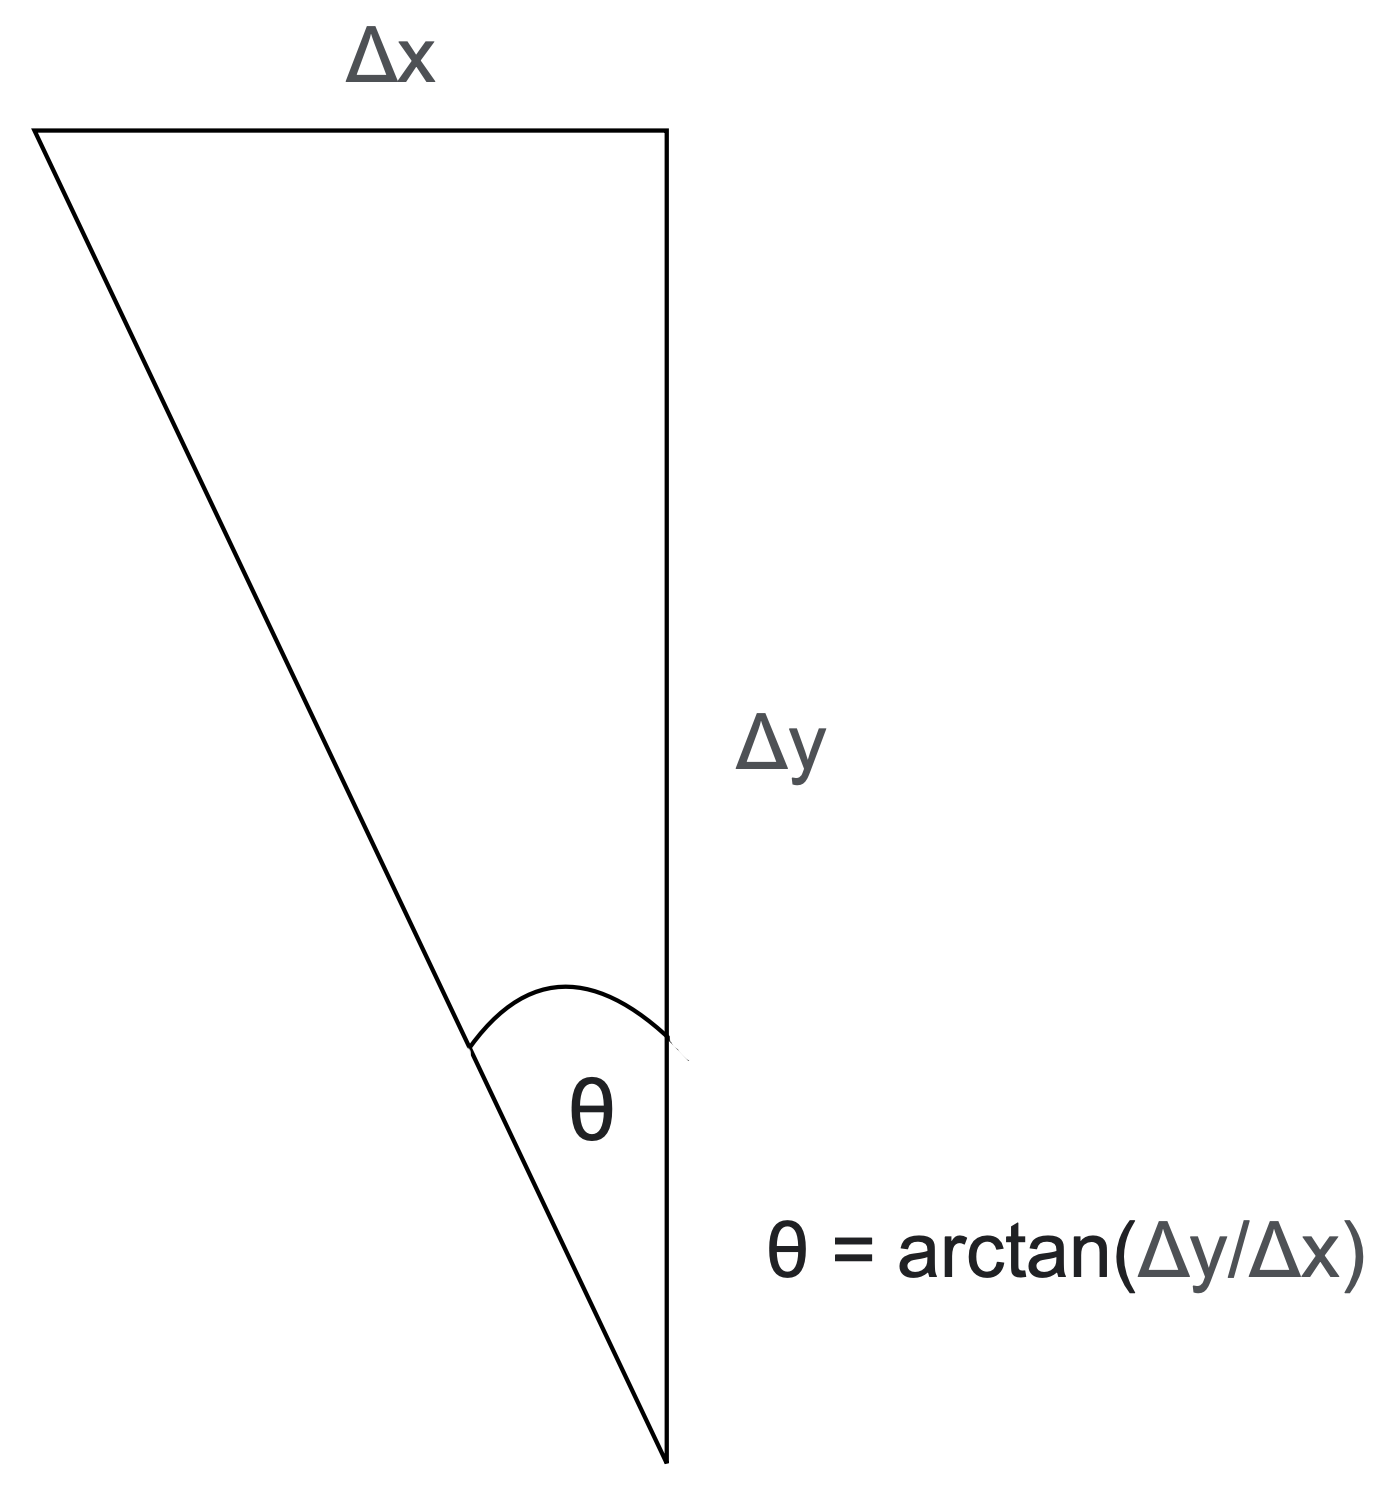
\includegraphics[width=0.5\textwidth]{Bilder/trig}
\end{center}


\begin{lstlisting}[language=Python]
delta_x = middle_x_top - middle_x_bottom
delta_y = middle_y_top - middle_y_bottom
angle_rad = np.arctan2(delta_y, delta_x)
angle_deg = np.degrees(angle_rad)
\end{lstlisting}


\subsection{Threshold}

\subsubsection*{Description}
The threshold is the region in which the middle of the lane can be before triggering a warning for lane correction. It stays static during the whole process. The threshold can be set automatically from the first frame in which the lane is detected or it can be manually set. 
\begin{center}
\includegraphics[width=0.8\textwidth]{Bilder/threshold}
\end{center}

\subsubsection*{Automatically Set}
\begin{lstlisting}[language=Python]
threshold_from_frame = True
threshold = 50 
\end{lstlisting}

When this variable is set to \textbf{True}, the line detection is performed until both lanes are detected. Then the threshold is set by translating the border lines along the x-axis by the threshold value:
\begin{lstlisting}[language=Python]
l_threshold_x_bottom = left_lane[0] + threshold
l_threshold_x_top = left_lane[2] + threshold

r_threshold_x_bottom = right_lane[0] - threshold
r_threshold_x_top = right_lane[2] - threshold
\end{lstlisting}

\subsubsection*{Manually Set}

\begin{lstlisting}[language=Python]
threshold_from_frame = False
threshold = 50 
threshold_x = 300
\end{lstlisting}

To manually set the threshold, set \textbf{threshold\_from\_frame} to \textbf{False}. The bottom of the threshold lines start at $x=\textbf{threshold\_x}$. Then they are translated by the \textbf{threshold} value (to left and right respectively). 
\\The top x values of the lines are set by using the slope formula: $y-y_1=m(x-x_1)$ where $x$ is the top of the line, so $x=x_1+(y-y_1)/m$. Note that $m=tan(\theta)$, where $\theta$ is the angle between the $x-axis$ and the line.

\begin{lstlisting}[language=Python]
angle_from_yaxis = 3
angle = np.radians(90 + angle_from_yaxis)  
y1 = height - 1 
y2 = int(height * 0.5)

l_threshold_x_bottom = threshold_x - threshold
l_threshold_x_top = l_threshold_x_bottom + (y2 - y1) / np.tan(angle)

r_threshold_x_bottom = threshold_x + threshold
r_threshold_x_top = r_threshold_x_bottom + (y2 - y1) / np.tan(-angle)
\end{lstlisting}
Therefore, with the variable \textbf{angle} it is possible to set the inclination of the threshold lines.


\subsection{Displacement}
\subsubsection*{Description}

The displacement of the robot across the lane is also important, as it helps to determine if the robot is already off track. This cannot be always determined by the rotation, since the lane can still be parallel to the robot even if the robot is off the lane. The point of reference to measure de displacement can be either the center of the $x-axis$ of the image or it can be set to be the middle of the threshold. This reference is represented as a small black line at bottom of the video.
\subsubsection*{Center of the Image}
\begin{lstlisting}[language=Python]
center_of_cam = True
\end{lstlisting}

When this parameter is set to \textbf{True}, the center of the image is taken by dividing the frame width by 2. 
\begin{lstlisting}[language=Python]
cam_width = int(video_capture.get(cv2.CAP_PROP_FRAME_WIDTH))
cam_center_x = cam_width // 2
\end{lstlisting}
\subsubsection*{Center of Threshold}
\begin{lstlisting}[language=Python]
center_of_cam = False
\end{lstlisting}

After setting this parameter to \textbf{False}, the \textbf{cam\_center\_x} is set to the $x$ coordinate of the bottom middle line (\textbf{middle\_x\_bottom}), or to \textbf{threshold\_x}, depending on whether the threshold is set automatically or manually.
\subsubsection*{Displacement Determination}

To calculate the displacement of the robot from the center of the lane, the distance along the $x-axis$ from the bottom of the center of the lane to the \textbf{cam\_center\_x} is calculated:

\begin{lstlisting}[language=Python]
distance = middle_x_bottom - cam_center_x
\end{lstlisting}

\begin{center}
\includegraphics[width=0.8\textwidth]{Bilder/final}
\end{center}

\subsubsection*{Final Code}

The code can be tested by running \textbf{lane\_detection.py}. 

\end{document}